% ------------------------------------------------------------------------
% ------------------------------------------------------------------------
% Trabalho de Graduação p/ o Curso de Engenharia Aeronáutica, UFU
% Autor: Filipe Guilherme Faria França
% Revisão: Prof. Dr. Pedro Assis
% O presente modelo foi obtido a partir do modelo desenvolvido por Alisson Lopes Furlani disponível na BU/UFSC.
% ------------------------------------------------------------------------
% ------------------------------------------------------------------------

\documentclass[
12pt,				% tamanho da fonte
%openright,			% capítulos começam em pág ímpar (insere página vazia caso preciso)
oneside,			% para impressão no anverso. Oposto a twoside
a4paper,			% tamanho do papel. 
chapter=TITLE,		% títulos de capítulos convertidos em letras maiúsculas
section=TITLE,		% títulos de seções convertidos em letras maiúsculas
%subsection=TITLE,	% títulos de subseções convertidos em letras maiúsculas
%subsubsection=TITLE,% títulos de subsubseções convertidos em letras maiúsculas
% -- opções do pacote babel --
english,			% idioma adicional para hifenização
brazil				% o último idioma é o principal do documento
]{abntex2}

\usepackage{configs/eca_ufsc_bnu} % personalização da ABNTEX2
\addbibresource{pos_textual/referencias.bib} % Seus arquivos de referências
\nocite{*} % Cita todas as referências

%---------------------------------------------------------------------------------------------
%--------- DADOS BÁSICOS DO TCC (Preencher todos) -------------------------------------
%---------------------------------------------------------------------------------------------
%Substituir 'Nome completo do autor' pelo seu nome.
\autor{Filipe Guilherme Faria França}
% FIXME Substituir 'Título do trabalho' pelo título da trabalho.
\titulo{IMPLEMENTAÇÃO DE CONTROLE ATIVO PARA SUPRESSÃO DE \textit{FLUTTER} DE UMA SEÇÃO TÍPICA BIDIMENSIONAL}
% Substituir 'Subtítulo (se houver)' pelo subtítulo da trabalho. 
% Se não houver subtítulo, basta deletar o texto.
\subtitulo{}
% Substituir 'Orientador' pelo nome do seu orientador.
\orientador{Prof. Dr. Pedro Augusto Queiroz de Assis}
% Se for orientado por uma mulher, comente a linha acima e descomente a linha a seguir.
% \orientador[Orientadora]{Orientadora, Dra.}
% Substituir 'XXXXXX' pelo nome do seu  coorientador. Caso não tenha coorientador, comente a linha a seguir.
% \coorientador{Prof. Coorientador, Dr.}
% Se for coorientado por uma mulher, comente a linha acima e descomente a linha a seguir.
% \coorientador[Coorientadora]{Coorientadora, Dra.}
\dia{11}
\mes{Outubro}
\ano{2022}
\local{Uberlândia}
\formacao{Bacharel em Engenharia Aeronáutica}
% Se for mulher, comente a linha acima e descomente a linha a seguir.
%\formacao{Engenheira de Controle e Automação}
\bancaa{Prof. Dr. Pedro Augusto Queiroz de Assis} %Primeiro membro da banca (normalmente o orientador).
\bancab{Prof. Dr. Tobias Souza Morais} %Segundo membro da banca
\bancac{Prof. Dr. Roberto de Souza Martins} %Terceiro membro da banca

%Resumo e palavras-chave do trabalho
\resumotcc{Será apresentada uma metodologia para projeto de um sistema de controle ativo para supressão de \textit{flutter} em sistemas aeroservoelásticos. \textit{Flutter} é um fenômeno de instabilidade aeroelástica dinâmica, cujo movimento oscilatório apresenta auto-excitação devido ao acoplamento dinâmico entre dois modos elásticos quaisquer do sistema. Essa instabilidade ocorre a partir de uma determinada velocidade, denominada velocidade de \textit{flutter}, em que as oscilações se tornam divergentes em relação a posição de equilíbrio do sistema, configurando um movimento instável. Devido à característica destrutiva do \textit{flutter}, são adotadas restrições de projeto para impedir que a velocidade de \textit{flutter} esteja dentro do envelope de operações. Mesmo em operações em velocidades inferiores a de \textit{flutter}, porém suficientemente próximas, podem ocorrer prejuízos ao desempenho de voo devido à elevada vibração da estrutura. Para mitigar os efeitos desse fenômeno no projeto e operação de aeronaves, pode ser adotado um sistema ativo de supressão de \textit{flutter}, que consiste em projetar uma lei de controle para atuar sobre o sistema regulando a vibração da estrutura com o objetivo de suprimir o \textit{flutter}. É nesse contexto que o presente trabalho se encaixa: Desenvolver um \glsxtrfull{AFS} para uma seção transversal de asa bidimensional com uma superfície de controle do tipo \textit{flap} no bordo de fuga. Para modelagem do sistema, os esforços aerodinâmicos dependentes da frequência reduzida são descritos empregando uma técnica conhecida como \glsxtrfull{RFA}, sendo considerados quatro polos de atraso para representar os efeitos não-estacionários da aerodinâmica. O modelo matemático é descrito utilizando uma representação no espaço de estados e então, adotado para projetar um controlador por realimentação de estados. Em particular, adotou-se a metodologia do \glsxtrfull{LQR} para projeto do ganho de realimentação de estados. Resultados de simulação mostraram uma velocidade de \textit{flutter} de $29,59$ m/s para o sistema estudado, um erro percentual de apenas $2\%$ em relação ao valor referência encontrado na literatura, indicando adequação da metodologia para modelagem no domínio do tempo realizada. Ademais, foram obtidos resultados que evidenciam a capacidade da estrutura em malha fechada proposta em estabilizar o sistema na condição de projeto, determinada como sendo o ponto de instabilidade dinâmica do sistema em malha aberta. Como consequência, também percebe-se o aumento da velocidade de \textit{flutter} do sistema em malha fechada, apesar de não haver garantia teórica para isso.
}
\palavraschave{Aeroelasticidade; Supressão ativa de \textit{flutter}; Análise no domínio do tempo; Aproximação da aerodinâmica não-estacionária por funções racionais}

%Abstract e keywords do trabalho
\abstracttcc{A design methodology for an active control system used to suppress \textit{flutter} in aeroservoelastic systems is presented. \textit{Flutter} is a dynamic aeroelastic instability phenomenon, whose oscilatory motion presents self-excitation due to the dynamic coupling between any two elastic modes of the system. This instability occurs from a certain velocity, called the \textit{flutter} velocity, in which the oscillations become divergent from the equilibrium point of the system, featuring an unstable movement. Due to the destructive characteristic of \textit{flutter}, design restrictions are adopted to prevent the \textit{flutter} velocity from being within the operational envelope. Even in operations at speeds below \textit{flutter}, but close enough, damage to flight performance may occur due to high vibration of the structure. To mitigate the effects of this phenomenon on aircraft design and operation, an active flutter suppression system can be adopted, which consists of designing a control law to act on the system by regulating the structure's vibration in order to suppress the \textit{ flutter}. It is in this context that the present work fits: Develop a \gls{AFS} for a two-dimensional wing cross section with a control surface located on the section's trailing edge. A technique known as \gls{RFA} is used to describe the reduced frequency-dependent aerodynamic loads in the time domain, in which four delay poles are assumed to represent the nonstationary effects of the aerodynamics. The mathematical model is described using a state-space representation. The control system was designed using this model via quadratic linear regulator methodology to design the state feedback gain. The estimated \textit{flutter} velocity for the studied system is found to be $29,59$ m/s, which indicates a percentage error of $2\%$ when compared to values from literature, showing the adequacy of the methodology implemented. Furthermore, the results obtained shows the ability of the proposed closed-loop structure to stabilize the system in the design condition, determined as the point of dynamic instability of the open-loop system. As a consequence, it can also be seen an increase in the \textit{flutter} speed of the closed-loop system, although there is no theoretical guarantee for this.}
\keywords{Aeroelasticity; Active \textit{flutter} suppression; Time-domain analysis; Rational Function Approximation of Aerodynamics}

%Agradecimentos (opcional). Caso não queira inserir, deixe em branco (\agradecimentostcc{} )
\agradecimentostcc{Primeiramente, gostaria de agradecer à minha família pelo suporte e amor proporcionado, especialmente aos meus pais, Ronaldo e Alessandra, por sempre me apoiarem durante as fases de descobrimento pessoal e profissional, e por me oferecerem o privilégio de me dedicar integralmente aos meus estudos.

Agradeço imensamente ao meu professor orientador Pedro Assis, pela orientação durante o desenvolvimento desse trabalho e pelo contato em sala de aula, partes fundamentais para que o projeto atingisse o nível desejado e em meu desenvolvimento como pesquisador.

À Universidade Federal de Uberlândia e à Faculdade de Engenharia Mecânica, expresso minha gratidão por proporcionarem o ambiente de formação em alto nível de qualidade, demonstrando a importância e necessidade da educação pública para o desenvolvimento do nosso país. Destaco o trabalho do professor e coordenador do curso de Engenharia Aeronáutica, Giuliano Venson, pelo suporte durante toda minha formação, disposto a tirar dúvidas e auxiliar como pôde nos processos internos, sempre tendo a formação dos estudantes como prioridade.

Gostaria de agradecer profundamente à equipe Tucano Aerodesign por proporcionar o meio no qual me tornei engenheiro. As dificuldades no desenvolvimento de projeto, os desafios a serem superados e as noites sem dormir construindo aeronaves junto de meus colegas de equipe, foram, sem dúvida, os momentos de maior aprendizado durante a graduação. Destaco aos membros integrantes das equipes de 2019, 2020 e 2022, por terem feito parte de minha jornada e me ajudado a crescer como engenheiro. Também agradeço ao professor orientador, Tobias Morais, por ter sido uma referência de engenharia aeronáutica durante toda minha graduação, sendo como orientador dos projetos de aerodesign, em sala de aula e na coorientação desse trabalho.

Também expresso meus sinceros agradecimentos a todos os amigos que Uberlândia me proporcionou e que fizeram dessa jornada uma experiência de vida, cheia de risadas, emoções e momentos inesquecíveis. Obrigado Aila Agostinho, Daniel Willbergher, Dimas Silvério, Guilherme Miyadaira, Lucas Alves, Lucas Cunha, Lucas Lutffalla e Luís Moura. Particularmente, agradeço à Amanda Leite, por trilhar ao meu lado essa jornada, sendo meu alicerce e fazendo dos dias felizes mais felizes e dos tristes suportáveis.
}

%Epígrafe (opcional). Caso não queira inserir, deixe em branco (\epigrafetcc{} )
\epigrafetcc{“Essencialmente, todos os modelos estão errados, \\ mas alguns são úteis.” (George E. P. Box)}

%Decatória (opcional). Caso não queira inserir, deixe em branco (\dedicatoriatcc{} )
\dedicatoriatcc{}

%Lista de quadros
%Além de figuras e tabelas, o TCC contém quadros? Caso afirmativo digite sim ou deixe em branco para não (\contemquadros{}).
\contemquadros{}

%Lista de siglas (opcional).
%Deseja incluir lista de abreviaturas e siglas? Caso afirmativo digite sim ou deixe em branco para não (\contemsiglas{}).
\contemsiglas{sim}

%Lista de símbolos (opcional).
%Deseja incluir lista de símbolos? Caso afirmativo digite sim ou deixe em branco para não (\contemsimbolos{}).
\contemsimbolos{sim}

%-------------------------FIM DOS DADOS BÁSICOS DO TCC--------------------------------------------

% ajusta espaçamento das listas itemize e enumerate
\setitemize{topsep=0pt,itemsep=0pt,leftmargin=\parindent+\labelwidth-\labelsep}
\setenumerate{topsep=0pt,itemsep=0pt,leftmargin=\parindent+\labelwidth-\labelsep}

% define a macro \Autoref to allow multiple references to be passed to \autoref
\makeatletter
\newcommand\Autoref[1]{\@first@ref#1,@}
\def\@throw@dot#1.#2@{#1}% discard everything after the dot
\def\@set@refname#1{%    % set \@refname to autoefname+s using \getrefbykeydefault
	\edef\@tmp{\getrefbykeydefault{#1}{anchor}{}}%
	\xdef\@tmp{\expandafter\@throw@dot\@tmp.@}%
	\ltx@IfUndefined{\@tmp autorefnameplural}%
	{\def\@refname{\@nameuse{\@tmp autorefname}s}}%
	{\def\@refname{\@nameuse{\@tmp autorefnameplural}}}%
}
\def\@first@ref#1,#2{%
	\ifx#2@\autoref{#1}\let\@nextref\@gobble% only one ref, revert to normal \autoref
	\else%
	\@set@refname{#1}%  set \@refname to autoref name
	\@refname~\ref{#1}% add autoefname and first reference
	\let\@nextref\@next@ref% push processing to \@next@ref
	\fi%
	\@nextref#2%
}
\def\@next@ref#1,#2{%
	\ifx#2@ e~\ref{#1}\let\@nextref\@gobble% at end: print e+\ref and stop
	\else, \ref{#1}% print  ,+\ref and continue
	\fi%
	\@nextref#2%
}
\makeatother

% Cria comando para referenciar Anexo automaticamente \refanexo
\newcommand{\refanexo}[1]{\hyperref[#1]{Anexo~\ref{#1}}}

% Define comandos para tabelas que permite ajustar o tamanho da coluna e manter alinhamento C, R ou L
%\newcommand{\PreserveBackslash}[1]{\let\temp=\\#1\let\\=\temp}
\newcolumntype{C}[1]{>{\centering\let\arraybackslash}m{#1}}
\newcolumntype{R}[1]{>{\RaggedLeft\let\arraybackslash}m{#1}}
\newcolumntype{L}[1]{>{\RaggedRight\let\arraybackslash}m{#1}}


% ---
% Filtering and Mapping Bibliographies
% ---
\DeclareSourcemap{
	\maps[datatype=bibtex]{
		% remove fields that are always useless
		\map{
			\step[fieldset=abstract, null]
			\step[fieldset=pagetotal, null]
			\step[fieldset=doi, null]
		}
		% remove URLs for types that are primarily printed
		\map{
			\pernottype{software}
			\pernottype{online}
			\pernottype{report}
			\pernottype{techreport}
			\pernottype{standard}
			\pernottype{manual}
			\pernottype{misc}
			\step[fieldset=url, null]
			\step[fieldset=urldate, null]
		}
		\map{
			\pertype{inproceedings}
			% remove mostly redundant conference information
			%\step[fieldset=venue, null]
			%\step[fieldset=eventdate, null]
			%\step[fieldset=eventtitle, null]
			% do not show ISBN for proceedings
			\step[fieldset=isbn, null]
			% Citavi bug
			%\step[fieldset=volume, null]
		}
	}
}
% ---

\preambulo
{%
	Projeto de Conclusão de Curso apresentado ao curso de Graduação em Engenharia Aeronáutica, da Faculdade de Engenharia Mecânica da Universidade Federal de Uberlândia como requisito para a obtenção~do~título~de~\imprimirformacao.
}
% ---

% ---
% Configurações de aparência do PDF final
% ---
% alterando o aspecto da cor azul
\definecolor{blue}{RGB}{41,5,195}
% informações do PDF
\makeatletter
\hypersetup{
	%pagebackref=true,
	pdftitle={\@title}, 
	pdfauthor={\@author},
	pdfsubject={\imprimirpreambulo},
	pdfcreator={LaTeX with abnTeX2},
	pdfkeywords={ufu, tcc, flutter, controle}, 
	colorlinks=true,       		        % false: boxed links; true: colored links
	linkcolor=black,%blue,          	% color of internal links
	citecolor=black,%blue,        		% color of links to bibliography
	filecolor=black,%magenta,      		% color of file links
	urlcolor=blue,
	bookmarksdepth=4
}
\makeatother
% ---

% Definição das siglas e símbolos

%----------------- LISTA DE ABREVIATURAS E SIGLAS--------------------------------------
\siglalista{GDL}{Grau de Liberdade}
\siglalista{GDLs}{Graus de Liberdade}
\siglalista{AFS}{Supressão ativa de \textit{flutter}, do inglês \textit{Active Flutter Supression}}
\siglalista{RFA}{Aproximação por Funções Racionais, do inglês \textit{Rational Function Approximation}}
\siglalista{MIMO}{Múltiplas entradas e múltiplas saídas, do inglês \textit{Multiple-Input Multiple-Output}}
\siglalista{LQR}{Regulador Linear Quadrático, do inglês \textit{Linear Quadratic Regulator}}
\siglalista{ZOH}{Segurador de Ordem Zero, do inglês \textit{Zero Order-Holder}}
\siglalista{ISA}{Atmosfera Internacional Padrão, do inglês \textit{International Standard Atmosphere}}
\siglalista{FAA}{Administração Federal de Aviação americana, do inglês \textit{Federal Aviation Administration}}
\siglalista{FEM}{Método dos Elementos Finitos, do inglês \textit{Finite Element Methods}}

%Para usar uma dada sigla ABC ao longo do texto\, use \glsxtrfull{ABC} se quiser apresentar a sigla e sua definição.
%Se quiser apresentar apenas a sigla\, use \gls{ABC}.


%-----------------SÍMBOLOS---------------------------------------------------------------
\simbololista{h}{\ensuremath{h}}{deslocamento linear vertical\, primeiro \gls{GDL}}
\simbololista{theta}{\ensuremath{\theta}}{rotação da seção em torno do eixo elástico\, segundo \gls{GDL}}
\simbololista{delta}{\ensuremath{\delta}}{Deflexão da superfície de controle}
\simbololista{m}{\ensuremath{m}}{Massa da seção bidimensional}
\simbololista{b}{\ensuremath{b}}{meia corda da seção típica bidimensional}
\simbololista{c}{\ensuremath{c}}{corda da seção típica bidimensional}
\simbololista{a}{\ensuremath{a}}{posição relativa do eixo elástico}
\simbololista{e}{\ensuremath{e}}{posição relativa do eixo de rotação da superfície de controle}
\simbololista{Stheta}{\ensuremath{S_{\theta}}}{Momento de massa estática em relação ao eixo elástico}
\simbololista{Itheta}{\ensuremath{I_{\theta}}}{Momento de inércia em relação ao eixo elástico}
\simbololista{fGDL}{\ensuremath{f_{r_{k}}}}{Frequência natural desacoplada do \gls{GDL} \ensuremath{r_{k} = \{ h, \theta \} }}
\simbololista{omegaGDL}{\ensuremath{\omega_{r_{k}}}}{Frequência natural\, em rad\, desacoplada do \gls{GDL} \ensuremath{r_{k} = \{ h, \theta \} }}
\simbololista{csiGDL}{\ensuremath{\xi_{r_{k}}}}{Amortecimento estrutural do \gls{GDL} \ensuremath{r_{k} = \{ h, \theta \}}}
\simbololista{SdeltaGDL}{\ensuremath{S_{\delta\,r_{k}}}}{Acoplamento inercial da superfície de controle ao \gls{GDL} \ensuremath{r_{k} = h, \theta}}
\simbololista{Voo}{\ensuremath{V_{\infty}}}{Velocidade do escoamento não perturbado}
\simbololista{rho}{\ensuremath{\rho}}{Densidade do ar na região do escoamento não perturbado}
\simbololista{qoo}{\ensuremath{q_{\infty}}}{Pressão dinâmica do escoamento não perturbado}
\simbololista{VOLF}{\ensuremath{V_{OLF}}}{Velocidade de \textit{flutter} em malha aberta}
\simbololista{VCLF}{\ensuremath{V_{CLF}}}{Velocidade de \textit{flutter} em malha fechada}
\simbololista{VLVI}{\ensuremath{V_{LVI}}}{Velocidade de instabilidade de baixa velocidade em malha fechada}
\simbololista{M}{\ensuremath{\boldsymbol{M}}}{Matriz de massa do sistema}
\simbololista{D}{\ensuremath{\boldsymbol{D}}}{Matriz de amortecimento do sistema}
\simbololista{K}{\ensuremath{\boldsymbol{K}}}{Matriz de rigidez do sistema}
\simbololista{Mc}{\ensuremath{\boldsymbol{M}_{c}}}{Matriz de acoplamento inercial entre os \gls{GDL}s elásticos e superfície de controle}
\simbololista{F}{\ensuremath{\boldsymbol{F}}}{Forças aplicadas ao sistema aeroelástico}
\simbololista{Fa}{\ensuremath{\boldsymbol{F}_{A}}}{Força aerodinâmica devido à deformação estrutural}
\simbololista{Fc}{\ensuremath{\boldsymbol{F}_{C}}}{Força aerodinâmica devido à deflexão da superfície de controle}
\simbololista{Fr}{\ensuremath{\boldsymbol{F}_{R}}}{Força de reação devido ao movimento da superfície de controle}
\simbololista{AICa}{\ensuremath{\boldsymbol{AIC}_{A}}}{Matriz de coeficientes de influência aerodinâmicos referente à deformação estrutural}
\simbololista{AICc}{\ensuremath{\boldsymbol{AIC}_{c}}}{Matriz de coeficientes de influência aerodinâmicos referente ao movimento da superfície de controle}
\simbololista{r}{\ensuremath{\boldsymbol{r}}}{Vetor de \gls{GDL}s do sistema aeroelástico}
\simbololista{k}{\ensuremath{k}}{Frequência reduzida}
\simbololista{Nx}{\ensuremath{N_{x}}}{Número de estados do modelo em espaço de estados}
\simbololista{Ny}{\ensuremath{N_{y}}}{Número de variáveis de saída do modelo em espaço de estados}
\simbololista{NGDL}{\ensuremath{N_{\gls{GDL}}}}{Número de \gls{GDL}s do sistema aeroelástico}
\simbololista{Nk}{\ensuremath{N_{k}}}{Número de valores de frequência reduzida}
\simbololista{NL}{\ensuremath{N_{L}}}{Número de termos de atraso da \gls{RFA}}
\simbololista{pn}{\ensuremath{p_{n}}}{Polo do termo \ensuremath{n} de atraso devido à \gls{RFA}}
\simbololista{Ai}{\ensuremath{\boldsymbol{A}_{i}}}{Matriz de aproximação \gls{RFA}\, sendo \ensuremath{i = 1,\ 2,\ \cdots,\ N_{L}+2}}
\simbololista{Xa}{\ensuremath{\boldsymbol{X}_{A,n}}}{Estados de atraso aerodinâmico devido à \gls{RFA}\, sendo \ensuremath{i = 1,\ 2,\ \cdots,\ N_{L}+2}}
\simbololista{A}{\ensuremath{\boldsymbol{A}}}{Matriz dinâmica do modelo completo em espaço de estados}
\simbololista{B}{\ensuremath{\boldsymbol{B}}}{Matriz de entrada do modelo completo em espaço de estados}
\simbololista{C}{\ensuremath{\boldsymbol{C}}}{Matriz de saída do modelo completo em espaço de estados}
\simbololista{x}{\ensuremath{\boldsymbol{x}}}{Vetor de estados do modelo completo}
\simbololista{y}{\ensuremath{\boldsymbol{y}}}{Vetor de saída do modelo completo}
\simbololista{uc}{\ensuremath{u_{c}}}{Entrada comandada do modelo completo como a deflexão desejada da superfície de controle}
\simbololista{Aae}{\ensuremath{\boldsymbol{A}_{ae}}}{Matriz dinâmica do modelo aeroelástico em espaço de estados}
\simbololista{Bae}{\ensuremath{\boldsymbol{B}_{ae}}}{Matriz de entrada do modelo aeroelástico em espaço de estados}
\simbololista{xae}{\ensuremath{\boldsymbol{x}_{ae}}}{Vetor de estados do modelo aeroelástico}
\simbololista{uae}{\ensuremath{\boldsymbol{u}_{ae}}}{Vetor de entrada do modelo aeroelástico}
\simbololista{Aac}{\ensuremath{\boldsymbol{A}_{ac}}}{Matriz dinâmica do modelo do atuador em espaço de estados}
\simbololista{Bac}{\ensuremath{\boldsymbol{B}_{ac}}}{Matriz de entrada do modelo do atuador em espaço de estados}
\simbololista{Phi}{\ensuremath{\Phi}}{Matriz dinâmica do modelo digital em espaço de estados}
\simbololista{Gamma}{\ensuremath{\Gamma}}{Matriz de entrada do modelo digital em espaço de estados}
\simbololista{Wx}{\ensuremath{\boldsymbol{W}_{x}}}{Matriz de peso da dinâmica de resposta no projeto do \gls{LQR}}
\simbololista{Wu}{\ensuremath{W_{u}}}{Matriz de peso da ação de controle no projeto do \gls{LQR}}
\simbololista{Gain}{\ensuremath{\boldsymbol{K}}}{Vetor de ganho de realimentação de estados}

%Para usar um dado símbolo SIMB ao longo do texto, use \gls{SIMB}.

% compila a lista de abreviaturas e siglas e a lista de símbolos
\makenoidxglossaries 

% compila o indice
\makeindex


% ------------------------------------------------------------------------------------------------
% --------------------------INÍCIO DO DOCUMENTO---------------------------------------------
% ------------------------------------------------------------------------------------------------
\begin{document}
	
	% Seleciona o idioma do documento (conforme pacotes do babel)
	% \selectlanguage{english}
	\selectlanguage{brazil}
	
	% Retira espaço extra obsoleto entre as frases.
	\frenchspacing 
	
	% Espaçamento 1.5 entre linhas
	\OnehalfSpacing
	
	% Corrige justificação
	%\sloppy
	

	%Elementos pré-textuais
	% \pretextual %a macro \pretextual é acionado automaticamente no início de \begin{document}
	% Capa, folha de rosto, ficha bibliografica, errata, folha de aprovação
	% Dedicatória, agradecimentos, epígrafe (opcional), resumos, listas
	% Capa
\imprimircapa


% Folha de rosto
% o * indica que haverá a ficha bibliográfica
 \imprimirfolhaderosto

% Inserir a ficha bibliografica
% http://ficha.bu.ufsc.br/
% \begin{fichacatalografica}
% 	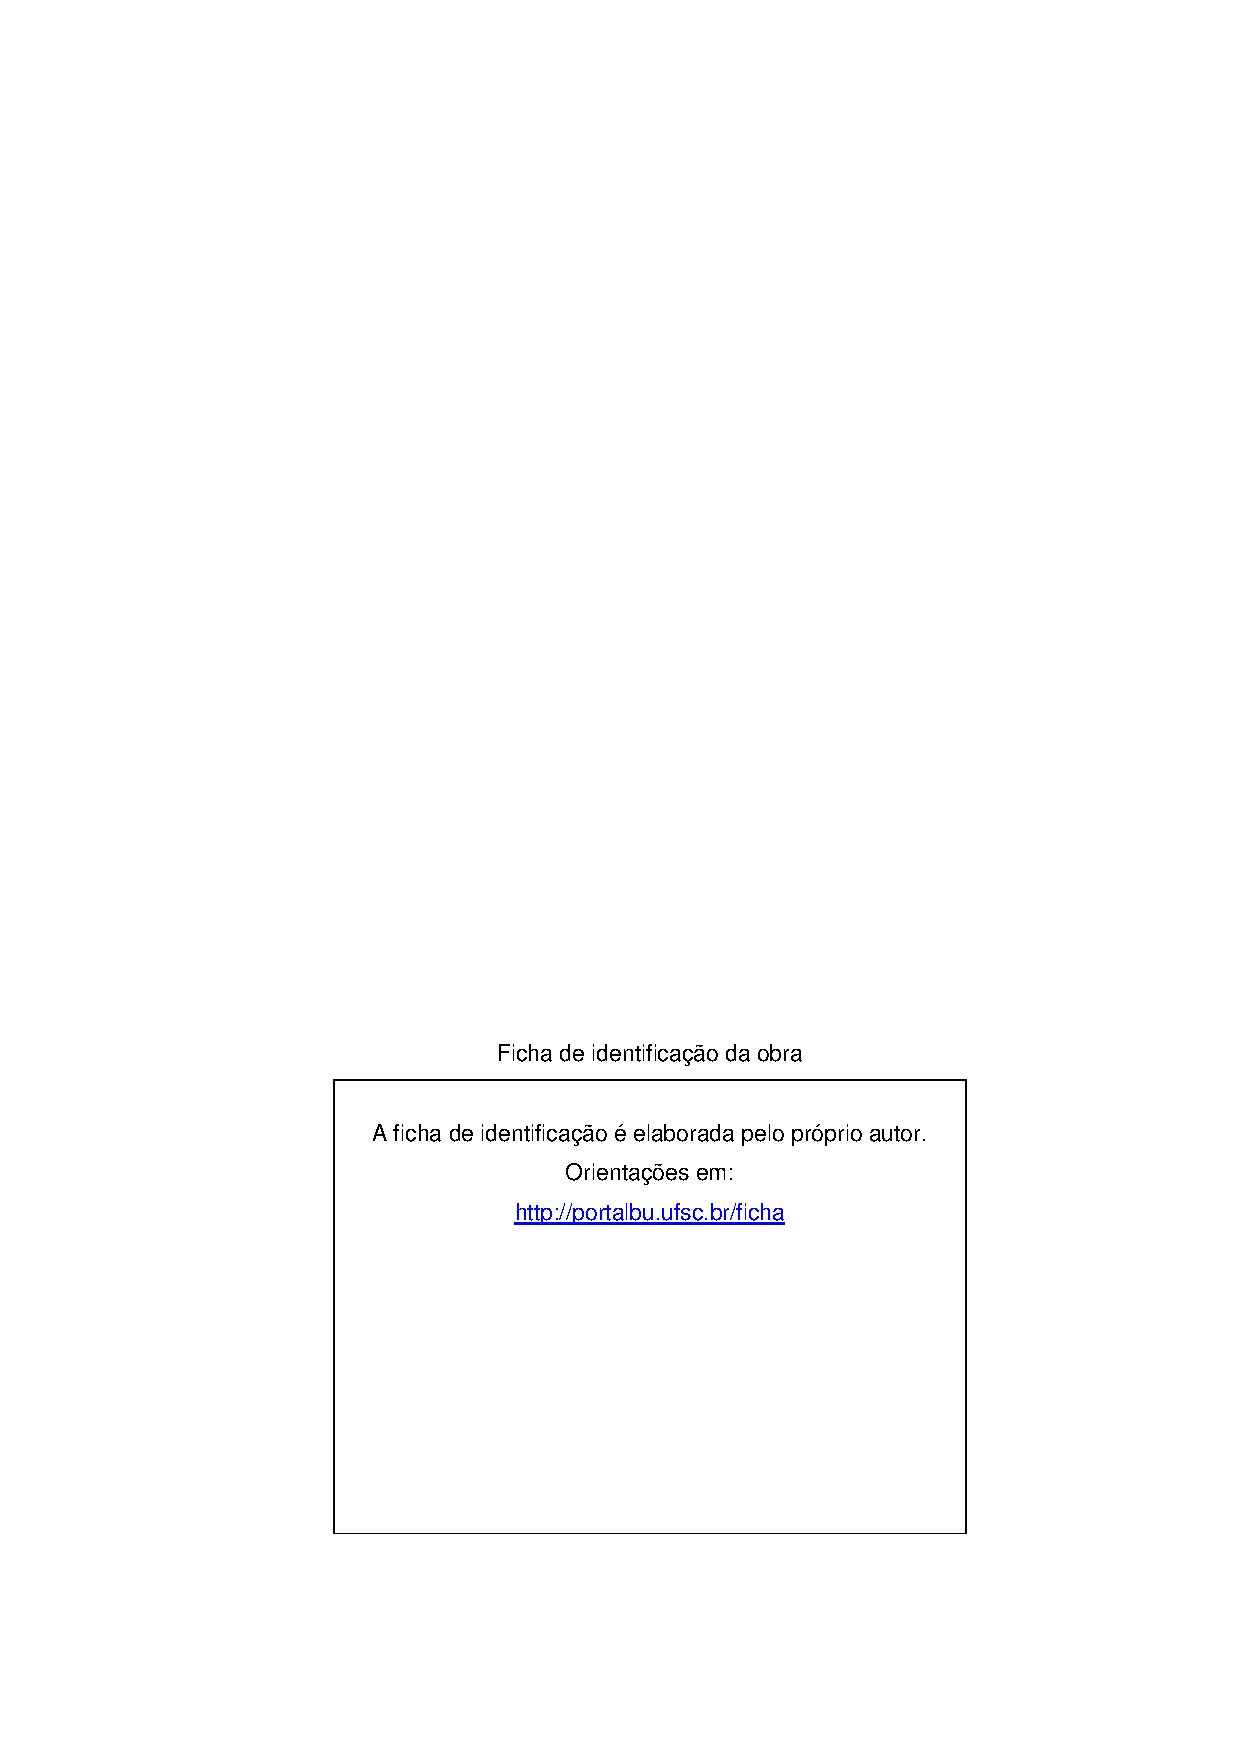
\includepdf{pre_textual/ficha_catalografica.pdf}
% \end{fichacatalografica}

% Inserir folha de aprovação
\begin{folhadeaprovacao}
	\OnehalfSpacing
	\centering
	\imprimirautor\\%
	\vspace{24pt}		
	\textbf{\imprimirtitulo}%
	\ifnotempty{\imprimirsubtitulo}{:~\imprimirsubtitulo}\\%
	\vspace*{31.5pt}%3\baselineskip
	\vspace*{\baselineskip}
	%\begin{minipage}{\textwidth}
	Este Trabalho de Conclusão de Curso foi julgado adequado para obtenção do Título de ``\imprimirformacao'' e aprovado em sua forma final pelo Curso de Graduação em Engenharia Aeronáutica.\\
	\vspace{12pt}
	\imprimirlocal, \imprimirdia~de~\imprimirmes~de~\imprimirano.\\
	
	\vspace*{24pt}
	\textbf{Banca Examinadora:}\\
	
	\vspace*{24pt}
	\assinatura{\OnehalfSpacing \imprimirbancaa }
	\vspace{6pt}
	Faculdade de Engenharia Mecânica\\Universidade Federal de Uberlândia
	
	\vspace*{24pt}
	\assinatura{\OnehalfSpacing \imprimirbancab}
	\vspace{6pt}
	Faculdade de Engenharia Mecânica\\Universidade Federal de Uberlândia
	
	\vspace*{24pt}
	\assinatura{\OnehalfSpacing \imprimirbancac}
	\vspace{6pt}
	Faculdade de Engenharia Mecânica\\Universidade Federal de Uberlândia
	
\end{folhadeaprovacao}

% Dedicatória
\ifnotempty{\imprimirdedicatoriatcc}{
{\raggedleft\vspace*{\fill}\Longstack[l]{%
    \imprimirdedicatoriatcc
}\par
}
}
% APAGAR O BLOCO ACIMA CASO QUEIRA, VOLTAR COM O P
%\begin{dedicatoria}
%	\vspace*{\fill}
%	\noindent
%	\begin{adjustwidth*}{}{5.5cm} 
%		\raggedleft       
%		\imprimirdedicatoriatcc
%	\end{adjustwidth*}
%\end{dedicatoria}
%}

% Agradecimentos
\ifnotempty{\imprimiragradecimentostcc}{
\begin{agradecimentos}
	\imprimiragradecimentostcc
\end{agradecimentos}
}

% Epígrafe
\ifnotempty{\imprimirepigrafetcc}{
{\raggedleft\vspace*{\fill}\Longstack[l]{%
    \imprimirepigrafetcc
}\par
}
}
\pagebreak
%\begin{epigrafe}
%	\vspace*{\fill}
%	\begin{adjustwidth*}{}{5.5cm} 
%	    \imprimirepigrafetcc
%    \end{adjustwidth*}
%\end{epigrafe}
%}


% Resumo
\setlength{\absparsep}{18pt} % ajusta o espaçamento dos parágrafos do resumo
\begin{resumo}
	%\SingleSpacing
	\imprimirresumotcc
	
	\textbf{Palavras-chave}: \imprimirpalavraschave
\end{resumo}
%
%
% Abstract
\selectlanguage{english}
\ifnotempty{\imprimirabstracttcc}{
\begin{abstract}
	%\SingleSpacing
	\imprimirabstracttcc
	
	\textbf{Keywords}: \imprimirkeywords
\end{abstract}
}
\pagebreak
%
\selectlanguage{brazil}
{%hidelinks
	\hypersetup{hidelinks}
	
	% inserir lista de figuras
	\pdfbookmark[0]{\listfigurename}{lof}
	\listoffigures*
	\cleardoublepage
	
	% inserir lista de quadros
%	\ifnotempty{\verificaquadros}{
%		\pdfbookmark[0]{\listofquadrosname}{loq}
%		\listofquadros*
%		\cleardoublepage
%	}
	
	% inserir lista de tabelas
	\pdfbookmark[0]{\listtablename}{lot}
	\listoftables*
	\cleardoublepage
	
	% inserir lista de abreviaturas e siglas (devem ser declarados no preambulo)
	\ifnotempty{\verificasiglas}{
	\imprimirlistadesiglas
	}
	
	% inserir lista de símbolos (devem ser declarados no preambulo)
	\ifnotempty{\verificasimbolos}{
	\imprimirlistadesimbolos
	}
	
	% inserir o sumario
	\pdfbookmark[0]{\contentsname}{toc}
	\tableofcontents*
	\cleardoublepage
%	
}%hidelinks


	% Elementos textuais
	\textual
	
	% 1 - Introdução
	% ----------------------------------------------------------
\chapter{Introdução}\label{cap:introducao}
% ----------------------------------------------------------

Um objetivo comum no desenvolvimento de aeronaves é a redução do peso estrutural, pois influencia diretamente na carga paga útil carregada e, consequentemente, no desempenho de mercado do projeto. Por outro lado, tal redução pode estar associada com a redução da rigidez estrutural dos componentes do veículo. Como resultado, efeitos aeroelásticos afetam o comportamento dinâmico da aeronave e o desempenho em voo e, por isso, devem ser considerados no ciclo de projeto.

O estudo de aeroelasticidade, dividido nas subáreas de aeroelasticidade estática e dinâmica, auxilia na investigação da resposta da estrutura devido ao escoamento e na influência das deformações da estrutura nos carregamentos aerodinâmicos \cite{book:Wright-Cooper}. A subárea estática visa descrever as deformações estruturais resultantes de carregamentos aerodinâmicos em regime permanente e avalia fenômenos como a divergência e reversão de comando. Já a aeroelasticidade dinâmica investiga o movimento vibratório da estrutura na presença de variações temporais nas forças aerodinâmicas, tendo como objeto de estudo principal um fenômeno conhecido como \textit{flutter} \cite{art:Collar-1978, art:Garrick&Reed-1981}. O \textit{flutter} é caracterizado como uma instabilidade dinâmica da estrutura, cujo movimento apresenta auto-excitação, ocorrendo quando há o acoplamento dinâmico entre dois modos elásticos quaisquer do sistema \cite{book:Wright-Cooper, art:Sun-2014}. Movimentos oscilatórios da estrutura ocorrem para todas as velocidades de voo da aeronave. Contudo, a partir de uma determinada velocidade, esses movimentos aumentam de amplitude continuamente, caracterizando um movimento dinâmico instável. Tal velocidade é denominada velocidade de \textit{flutter} \cite{book:Wright-Cooper}.

Efeitos aeroelásticos afetam o desenvolvimento da aviação antes mesmo do primeiro voo de uma aeronave propelida acontecer. É discutido por \textcite{book:Bisplinghoff} que a causa atribuída à segunda falha do protótipo Aerodrome A, Figura \ref{fig:cap1:Aerodrom-Langley}, desenvolvido por Samuel Langley em 1903, ocorreu devido a problemas aeroelásticos, mais especificamente ao efeito de divergência. Problemas de divergência nas superfícies aerodinâmicas foram muito comuns durante os avanços da aviação durante a Primeira Guerra Mundial e, como abordado por \textcite{art:Collar-1978}, esses problemas eram solucionados simplesmente aumentando a rigidez estrutural.

\begin{figure}[ht]
    \centering
    \caption{Foto das tentativas de voo do protótipo Aerodrome A, no dia 07 de Outubro de 1903. Foram realizadas duas tentativas de voo, nas quais a aeronave foi catapultada de uma plataforma no rio Potomac, EUA. Em ambas tentativas o protótipo caiu no rio.}
    \noindent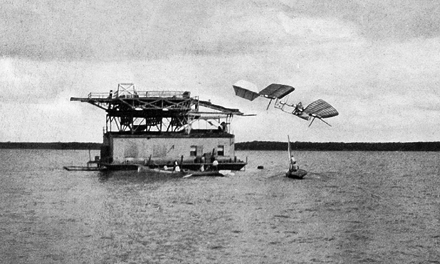
\includegraphics[width=\textwidth]{trabalho-graduacao/capitulos/figures/cap_1/Aerodrome-Langley.jpeg}
    \label{fig:cap1:Aerodrom-Langley}
\end{figure}

A primeira ocorrência documentada de \textit{flutter} afetando o voo de uma aeronave ocorreu em 1916 com o bombardeiro  Handley Page O/400 \cite{art:Le-2015}. Nesse caso, a aeronave apresentou oscilação extrema da empenagem, causando deformação da fuselagem e impactando a dinâmica do voo devido ao movimento dos profundores se tornarem assimétricos graças à deformação. Um exemplo de \textit{flutter} causando dano estrutural fora da aviação, é o colapso da ponte de Tacoma Narrows no dia 7 de Novembro de 1940 \cite{art:Billah-1990}. O fenômeno foi induzido por ventos de alta velocidade, chegando a aproximadamente $18,9$ m/s, o que levou a vibrações de extrema magnitude, como mostrado na Figura \ref{fig:cap1:Tacoma-Bridge}.

\begin{figure}[ht]
    \centering
    \caption{Fotos da ponte Tacoma Narrows, EUA colapsando em Novembro de 1940 devido ao \textit{flutter}; (\ref{fig:Tacoma-Oscilacao-01}) e (\ref{fig:Tacoma-Oscilacao-02}) mostram a amplitude das oscilações da seção central da ponte vista de cima, (\ref{fig:Tacoma-Oscilacao-03}) mostra a oscilação vista de fora da ponte, e (\ref{fig:Tacoma-Colapso}) apresenta uma foto após o colapso estrutural}
    \begin{subfigure}[t]{0.49\textwidth}
        \centering
        \caption{}
        \noindent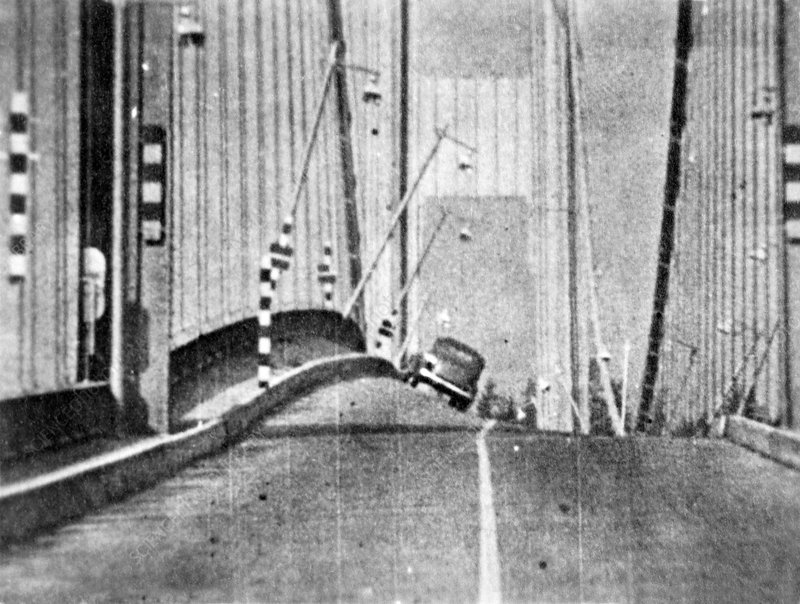
\includegraphics[width=\textwidth]{trabalho-graduacao/capitulos/figures/cap_1/Tacoma-Bridge-01.jpg}
        \label{fig:Tacoma-Oscilacao-01}
    \end{subfigure}
    \begin{subfigure}[t]{0.49\textwidth}
        \centering
        \caption{}
        \noindent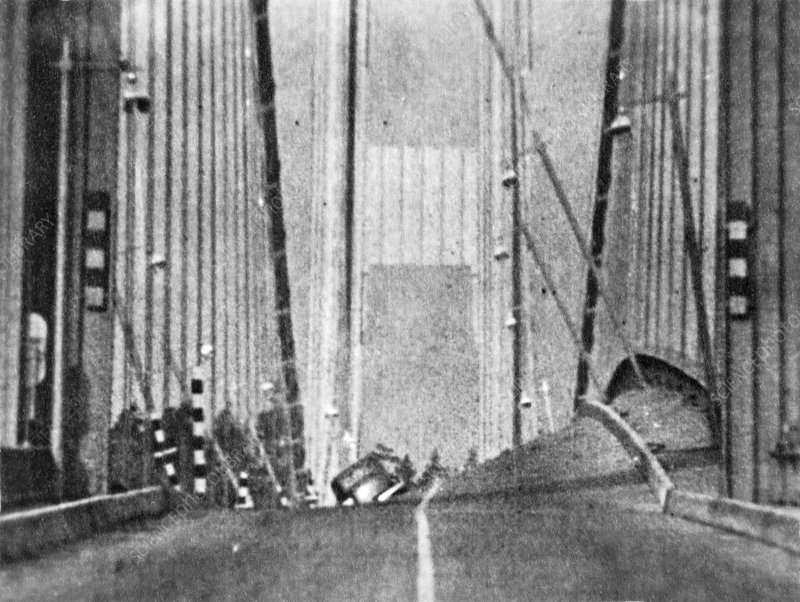
\includegraphics[width=\textwidth]{trabalho-graduacao/capitulos/figures/cap_1/Tacoma-Bridge-02.jpg}
        \label{fig:Tacoma-Oscilacao-02}
    \end{subfigure} \\
    \begin{subfigure}[t]{0.49\textwidth}
        \centering
        \noindent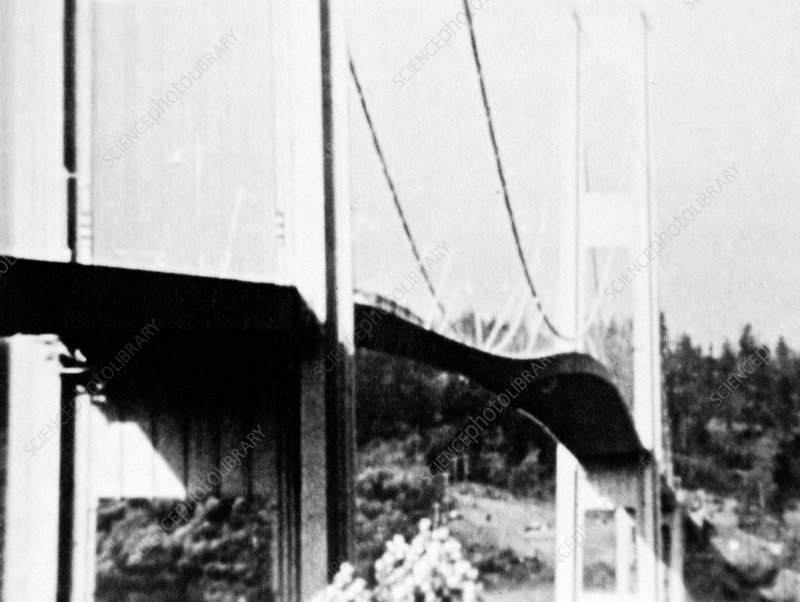
\includegraphics[width=\textwidth]{trabalho-graduacao/capitulos/figures/cap_1/Tacoma-Bridge-03.jpg}
        \caption{}
        \label{fig:Tacoma-Oscilacao-03}
    \end{subfigure}
    \begin{subfigure}[t]{0.49\textwidth}
        \centering
        \noindent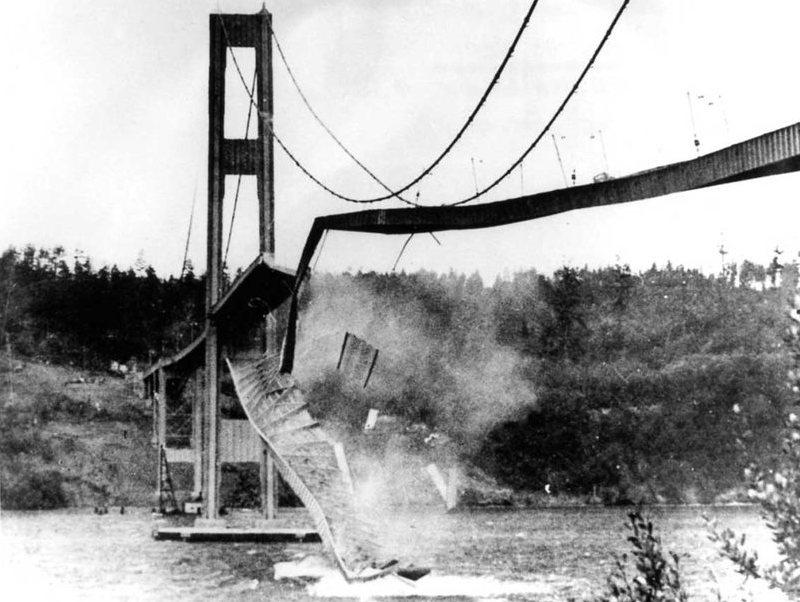
\includegraphics[width=\textwidth]{trabalho-graduacao/capitulos/figures/cap_1/Tacoma-Bridge-04.png}
        \caption{}
        \label{fig:Tacoma-Colapso}
    \end{subfigure}
        \label{fig:cap1:Tacoma-Bridge}
\end{figure}

Para evitar danos estruturais associados ao fenômeno do \textit{flutter}, restrições são consideradas no projeto aeronáutico visando impedir que a velocidade na qual essa instabilidade ocorre esteja dentro do envelope de operações, como, por exemplo, as restrições impostas pela \glsxtrfull{FAA} para projeto aeronáutico pelas normas 14 C.F.R § 23 e 25. Tais restrições se refletem no acréscimo de massa estrutural, afim de mitigar possíveis problemas encontrados no decorrer do desenvolvimento. Além disso, o envelope de voo é estritamente mantido para que a aeronave não se aproxime da velocidade de \textit{flutter} \cite{art:Sun-2014}. Com o objetivo de propor formas de mitigar os problemas decorrentes desse fenômeno, foram propostas na literatura técnicas de controle ativo para supressão de \textit{flutter}, \glsxtrfull{AFS}. O uso de \gls{AFS} em projetos aeronáuticos pode ser dado tanto no início do desenvolvimento, quanto em estágios mais avançados. Quando utilizado em etapas iniciais, essa técnica pode acarretar em redução do peso vazio projetado e melhoria no desempenho da aeronave \cite{art:Livne-1999}. Em projetos já em andamento, o \gls{AFS} pode ser utilizada visando evitar acréscimos de massa ou reprojeto estrutural e aerodinâmico, quando deparado com problemas aeroelásticos \cite{art:Livne-2018}.

O emprego de \gls{AFS} visa aumentar a velocidade na qual a instabilidade ocorre. Diversos trabalhos foram realizados visando investigar o desempenho de sistemas \gls{AFS} em melhorar a estabilidade do sistema. Em \textcite{art:Sun-2014}, um aumento de $30\%$ na velocidade de \textit{flutter} foi obtido em simulação, para um modelo aeroservoelástico (composição entre os modelos aeroelástico e do atuador) desenvolvido no domínio do tempo da asa de \textit{Goland}, conhecida na literatura. O sistema \gls{AFS} utilizado pelo autor é composto por uma superfície de controle alocada no bordo de fuga e foi projetado empregando o controle preditivo baseado em modelo. Investigações experimentais envolvendo o \textit{flutter}, utilizando ensaios em túnel de vento de uma asa, foram realizadas por \textcite{art:NASA1367}. Os resultados obtidos foram comparados com um modelo desenvolvido para a asa ensaiada no domínio do tempo empregando a técnica de \glsxtrfull{RFA} para inclusão dos termos aerodinâmicos. Foi observado pelo autor que a utilização da RFA possibilitou descrever adequadamente o comportamento dinâmico do sistema quando comparado com os resultados experimentais observados. Uma comparação entre resultados experimentais e de simulação também foi apresentada por \textcite{art:Huang-2015}, que obteve um aumento de $8\%$ na velocidade de \textit{flutter} para uma asa tridimensional com \gls{AFS}.

Nesse contexto, o presente trabalho envolve o desenvolvimento de um controlador para aumento da velocidade de \textit{flutter} de uma seção típica de aerofólio bidimensional. Com tal propósito, é realizado a modelagem matemática do sistema no domínio do tempo com uma representação no espaço de estados, sendo os esforços aerodinâmicos incluídos no modelo a partir da técnica \gls{RFA} \cite{book:Wright-Cooper, art:NASA1367, art:NASA2776, art:RogerRFA1977}. A lei de controle para supressão de \textit{flutter} foi do tipo realimentação de estados, sendo o vetor de realimentação projetado utilizando o conhecido regulador linear quadrático, \glsxtrfull{LQR}. Nesta estratégia, o controlador é projetado de modo a minimizar uma função de custo quadrática composta pelo desvio dos estados da sua posição regulada e da maginute da ação de controle, considerando um modelo linear do sistema. Para o caso particular de tempo final infinito, a solução do problema do \gls{LQR} é um vetor de realimentação de estados, que é calculado a partir da equação de Riccati, e depende de matrizes de ajuste que ponderam entre a velocidade de resposta e o esforço de controle \cite{book:Franklin}. É possível demonstrar que tal técnica de projeto resulta em margens de estabilidade interessantes. Mais precisamente, o \gls{LQR} resulta em uma margem de ganho acima de 6 dB e de fase de $60^{\circ}$ \cite{art:Anderson-1966, book:Anderson-1971}, justificando o emprego dessa abordagem.

Diante do exposto, o restante do trabalho foi dividido e será apresentado no decorrer do presente relatório seguindo a divisão em quatro partes, sendo:

\begin{itemize}
    \item O Capítulo 2 abordará a descrição do sistema aeroservoelástico e o desenvolvimento matemático do modelo. Incluir-se-ão os modos aeroelásticos associados aos \glsxtrfull{GDLs} para avaliar as margens de estabilidade do sistema;
    \item Em seguida, no Capítulo 3, o desenvolvimento da lei de controle por realimentação de estado será apresentado;
    \item No Capítulo 4 serão apresentados os resultados de simulação, discutindo-se a eficácia da abordagem da lei de controle na supressão de \textit{flutter};
    \item Por fim, no Capítulo 5 são listadas as conclusões das investigações numéricas e elencadas propostas de trabalhos futuros para continuidade do desenvolvimento.
\end{itemize}

% ----------------------------------------------------------

	
	% 2 - Modelo Aeroelástico
	% ----------------------------------------------------------
\chapter{Modelo Aeroservoelástico}\label{cap:modelo}
% ----------------------------------------------------------
A modelagem matemática do sistema aeroservoelástico deve ser realizada de forma a descrever a interação das forças inercias, deformações estruturais e carregamentos aerodinâmicos. Grande parte dos problemas aeroelásticos são abordados a partir de uma metodologia que utiliza uma descrição no domínio da frequência para os fenômenos dinâmicos, o que representa uma vantagem já que modelagens clássicas para determinação dos esforços aerodinâmicos apresentam os resultados em função da frequência reduzida \cite{book:Wright-Cooper}. Entretanto, essa descrição considera somente movimentos totalmente desenvolvidos, isto é, representados por sinais harmônicos e, apesar de apresentar grande representatividade de modelagem de movimentos oscilatórios, o estudo do comportamento transitório não é possível a partir desta metodologia \cite{book:Fung}.

Com o objetivo de considerar o comportamento transitório causado por condições iniciais não-nulas, entradas forçadas e perturbações, uma abordagem no domínio do tempo é necessária. Para isso, os esforços aerodinâmicos, cuja dependência da frequência representa os efeitos não estacionários, devem ser tratados de forma que tal dependência possa ser representada no domínio do tempo \cite{book:Wright-Cooper}. A modelagem no tempo pode ser feita utilizando uma representação no espaço de estados, o que representa vantagens na aplicação do modelo em projeto de leis de controle, sobretudo na realimentação de estados, que é a técnica a ser adotada no presente trabalho.

Neste capítulo será feita a modelagem do sistema de estudo, composto de uma seção transversal bidimensional de asa com \textit{flap} no bordo de fuga atuando como superfície de controle, vide Figura \ref{fig:cap2:sistema-fisico}. Em particular, serão desenvolvidas as equações do movimento que descrevem o sistema e, posteriormente, os esforços generalizados (carregamentos aerodinâmicos) são tratados utilizando uma metodologia designada \glsxtrfull{RFA}, baseada em \textcite{art:RogerRFA1977}. Por fim, as equações do movimento e a aproximação dos termos aerodinâmicos são integradas, obtendo o modelo completo no espaço de estados.

% ----------------------------------------------------------

% ----------------------------------------------------------
\section{Descrição do Sistema}\label{sec:descricao-sistema}
% ----------------------------------------------------------

O objeto de estudo do presente trabalho é um modelo com dois \gls{GDL}s, representando uma seção bidimensional típica de uma superfície aerodinâmica, com a presença de uma superfície de controle no bordo de fuga (Figura \ref{fig:cap2:sistema-fisico}).

\begin{figure}[ht]
    \centering
    \caption{Seção típica bidimensional com dois \gls{GDL}s}
    \noindent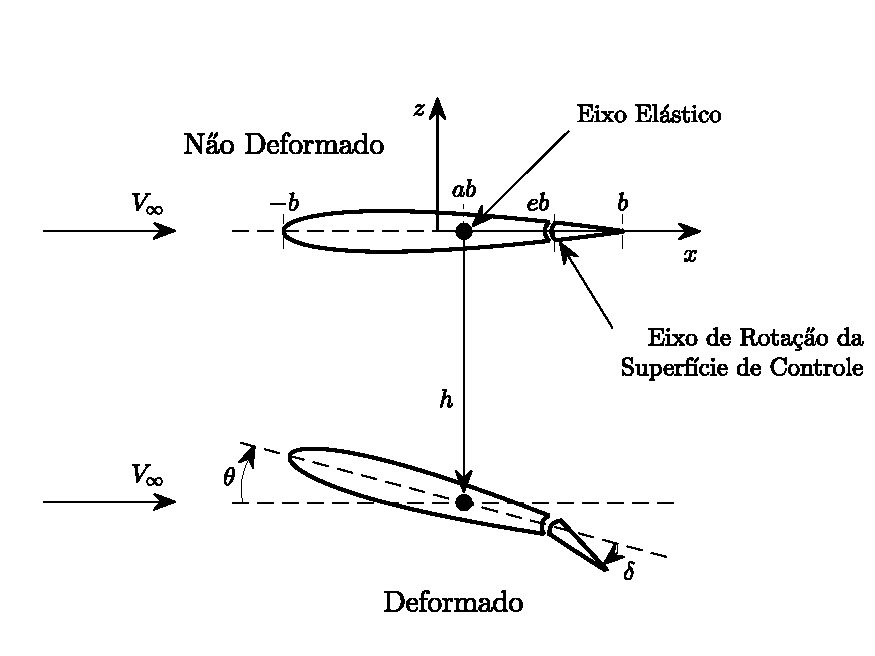
\includegraphics[width=\textwidth]{trabalho-graduacao/capitulos/figures/cap_2/secao-tipica.pdf}
    \label{fig:cap2:sistema-fisico}
\end{figure}

O referencial adotado contém a origem na posição de meia corda da seção, com os eixos conforme apresentados na figura. Os \gls{GDL}s que descrevem os movimentos de interesse são

\begin{itemize}
    \item Deslocamento linear vertical, \gls{h};
    \item Rotação da seção bidimensional em torno do eixo elástico, \gls{theta}.
\end{itemize}

Como já mencionado, o sistema é controlado por uma superfície de controle do tipo \textit{flap}, localizada no bordo de fuga da seção bidimensional podendo rotacionar em torno do eixo de rotação da superfície, localizado à uma distância $e$ em relação à origem, e representado pela variável $\gls{delta}$. Considerou-se que a dinâmica dessa superfície é determinada exclusivamente pela ação do atuador sobre a mesma, ou seja, negligenciaram-se os efeitos aeroelásticos associados ao seu movimento.

Além dos \gls{GDL}s e da superfície de controle, a Figura \ref{fig:cap2:sistema-fisico} apresenta os parâmetros físicos e geométricos que impactam na descrição do sistema. As indicações apresentadas na imagem se referem aos seguintes parâmetros:

\begin{itemize}
    \item \gls{Voo} representa a velocidade do escoamento não perturbado;
    \item \gls{b} é o valor da semi-corda da seção típica, a corda total é dada como \gls{c} $ = 2b$;
    \item \gls{a} é a posição relativa do eixo elástico a partir da posição de corda média, isto é, da origem do sistema de referência adotado;
    \item O eixo de rotação da superfície está a uma posição relativa igual a \gls{e} a partir da posição de corda média.
\end{itemize}


% ----------------------------------------------------------
\section{Equações do Movimento}\label{sec:equacoes-movimento}

Para o desenvolvimento das equações do movimento que descrevem o sistema aeroelástico, deve-se realizar o balanço dos esforços de inércia, aerodinâmicos, elásticos e os esforços externos que excitam o sistema \cite{book:Fung}. A forma geral para as equações que representam o sistema aeroelástico é definida segundo \textcite{book:Wright-Cooper}, como

\begin{equation} \label{eq:equacao-dinamica}
    \gls{M}\ddot{\gls{r}} +  \gls{D}\dot{\gls{r}} + \gls{K}\gls{r} = \boldsymbol{F}
\end{equation}

\noindent na qual as matrizes \gls{M} $\in \mathbb{R}^{\gls{NGDL} \times \gls{NGDL}}$, \gls{D} $\in \mathbb{R}^{\gls{NGDL} \times \gls{NGDL}}$ e \gls{K} $\in \mathbb{R}^{\gls{NGDL} \times \gls{NGDL}}$ são as matrizes de massa, amortecimento e rigidez do sistema, respectivamente. O vetor \gls{r} é o vetor de \gls{GDL}s, definido como,

\begin{equation} \label{eq:gdls}
    \gls{r} = \begin{bmatrix}
        \gls{h} & \gls{theta}
    \end{bmatrix}^{T}
\end{equation}

A dependência com o tempo de cada termo em \eqref{eq:equacao-dinamica} e \eqref{eq:gdls} foi omitida para claridade do texto. Em \eqref{eq:equacao-dinamica}, as parcelas $\gls{M}\ddot{\gls{r}}$, $\gls{D}\dot{\gls{r}}$ e $\gls{K}\gls{r}$ são, respectivamente as forças inerciais, de amortecimento e elástica referentes aos \gls{GDL}s do modelo estrutural, esses que são representados por \gls{r}. Mais ainda, \gls{F} representa as forças externas atuando sobre esses \gls{GDL}s. Neste trabalho serão consideradas as parcelas devido: aos esforços aerodinâmicos induzidos pela deformação estrutural, \gls{Fa}, à aerodinâmica imposta pela deflexão da superfície de controle, \gls{Fc} e ao esforço de reação inercial do movimento da superfície de controle, \gls{Fr}. Matematicamente, 

\begin{equation} \label{eq:forcas-aplicadas}
    \gls{F} = \gls{Fa} + \gls{Fc} + \gls{Fr}
\end{equation}

As parcelas de força provenientes de esforços aerodinâmicos devem ser calculadas contabilizando o efeito não estacionário do comportamento. Como discutido por \textcite{book:Wright-Cooper}, usualmente tais esforços são definidos no domínio da frequência utilizando-se da definição de frequência reduzida $k$, dada por

\begin{equation}\label{eq:Frequencia-reduzida}
    i\gls{k} = \frac{s\gls{b}}{\gls{Voo}}
\end{equation}

\noindent em que $s$ é a variável de Laplace, $i = \sqrt{-1}$ é a variável complexa e \gls{Voo} e \gls{b} representam a velocidade do escoamento não perturbado e o comprimento característico do modelo, respectivamente.

A força aerodinâmica devido à deformação estrutural pode ser dada por

\begin{equation} \label{eq:forca-aerodinamica}
    \gls{Fa} = \gls{qoo}\gls{AICa}(i\gls{k})\gls{r}
\end{equation}

\noindent sendo $\gls{qoo}=\frac{\gls{rho} \gls{Voo}}{2}$. O desenvolvimento matemático para obtenção de \eqref{eq:forca-aerodinamica} pode ser encontrado em \textcite{ZAERO-Theoretical-Manual:2017}. O termo $\gls{AICa} \in \mathbb{C}^{\gls{NGDL} \times \gls{NGDL}}$ em \eqref{eq:forca-aerodinamica} é a matriz de coeficientes de influência aerodinâmica, que é função da frequência reduzida e descreve o comportamento aerodinâmico não estacionário, como definida por \textcite{book:Wright-Cooper}. De maneira similar, a força aerodinâmica induzida pela deflexão da superfície de controle é dada por

\begin{equation} \label{eq:forca-superficie-controle}
    \gls{Fc} = \gls{qoo}\gls{AICc}(i\gls{k})\gls{delta}
\end{equation}

\noindent em que $\gls{delta}$ representa o ângulo de deflexão e $\gls{AICc} \in \mathbb{C}^{\gls{NGDL} \times 1}$ é a parcela da matriz de coeficientes de influência aerodinâmica referente à superfície de controle.

Estruturalmente, o movimento da superfície de controle induz uma força de reação na estrutura (aplicada nos \gls{GDL}s) definida por

\begin{equation} \label{eq:forca-reacao-superficie-controle}
    \gls{Fr} = -\gls{Mc}\ddot{\gls{delta}}
\end{equation}

\noindent sendo $\gls{Mc} \in \mathbb{R}^{\gls{NGDL} \times 1}$ a matriz de acoplamento inercial entre os \gls{GDL}s elásticos e da superfície de controle.

Assim, a equação \eqref{eq:equacao-dinamica} pode ser reescrita substituindo-se as forças definidas em \eqref{eq:forca-aerodinamica}, \eqref{eq:forca-superficie-controle} e \eqref{eq:forca-reacao-superficie-controle} resultando em

\begin{equation} \label{eq:equacao-dinamica2}
    \gls{M}\ddot{\gls{r}} +  \gls{D}\dot{\gls{r}} + \gls{D}\gls{r} = \gls{qoo}\gls{AICa}(i\gls{k})\gls{r} +  \gls{qoo}\gls{AICc}(i\gls{k})\gls{delta} - \gls{Mc}\ddot{\gls{delta}}
\end{equation}


Então, as equações do movimento de \eqref{eq:equacao-dinamica2} podem ser expressas de forma concisa no formato matricial como

\begin{equation} \label{eq:equacao-dinamica-final}
    \begin{bmatrix}
        \gls{M} & \gls{Mc}
    \end{bmatrix}
    \begin{bmatrix}
        \ddot{\gls{r}} \\ \ddot{\gls{delta}}
    \end{bmatrix}
    +
    \begin{bmatrix}
        \gls{D} & \boldsymbol{0}
    \end{bmatrix}
    \begin{bmatrix}
        \dot{\gls{r}} \\ \dot{\gls{delta}}
    \end{bmatrix}
    +
    \begin{bmatrix}
        \gls{K} & \boldsymbol{0}
    \end{bmatrix}
    \begin{bmatrix}
        \gls{r} \\ \gls{delta}
    \end{bmatrix}
    =
    \gls{qoo}\begin{bmatrix}
        \gls{AICa} & \gls{AICc}
    \end{bmatrix}
    \begin{bmatrix}
        \gls{r} \\ \gls{delta}
    \end{bmatrix}
\end{equation}

Para a seção bidimensional, as matrizes estruturais que definem o sistema, isto é $\gls{M}$, $\gls{D}$, $\gls{K}$ e $\gls{Mc}$, podem ser encontradas resolvendo as Equações de Lagrange para o sistema, conforme mostrado por \textcite{book:Wright-Cooper}, resultando em

\begin{equation}\label{eq:matriz-massa}
    \gls{M} = \begin{bmatrix}
        \gls{m} & S_{\theta} \\ S_{\theta} & I_{\theta} 
    \end{bmatrix}
\end{equation}

\begin{equation}\label{eq:matriz-amortecimento}
    \gls{D} = \begin{bmatrix}
        \xi_{h}(2m\omega_{h}) & 0 \\ 0 & \xi_{\theta}(2I_{\theta}\omega_{\theta}) 
    \end{bmatrix}
\end{equation}

\begin{equation}\label{eq:matriz-rigidez}
    \gls{K} = \begin{bmatrix}
        2m\omega^{2}_{h} & 0 \\ 0 & I_{\theta}\omega^{2}_{\theta} 
    \end{bmatrix}
\end{equation}

\begin{equation}\label{eq:matriz-acoplamento-inercial}
    \gls{Mc} = \begin{bmatrix}
        S_{\delta,h} \\ S_{\delta,\theta} 
    \end{bmatrix}
\end{equation}

\noindent sendo $\gls{csiGDL}$ e $\gls{omegaGDL}$, para $r_{k} = \{ \gls{h}, \ \gls{theta} \}$, respectivamente, amortecimentos e frequências naturais dos \gls{GDL}s desacoplados. Os parâmetros $S_{\theta}$ e $I_{\theta}$ representam o momento de massa estática e de inércia em relação ao eixo elástico, como definido por \textcite{book:Fung}. Além disso, $S_{\delta,h}$ e $S_{\delta,\theta}$ são os parâmetros de acoplamento inercial do movimento da superfície de controle aos \gls{GDL}s.

Vale comentar que, em \eqref{eq:equacao-dinamica-final}, omitiu-se a dependência da frequência reduzida das matrizes aerodinâmicas \gls{AICa} e \gls{AICc}. Porém, destaca-se que, apesar das equações do movimento serem apresentadas no domínio do tempo, os efeitos não-estacionários das matrizes aerodinâmicas devem ser expressos de forma a modelar no tempo os termos dependentes da frequência reduzida, o que será abordado na seção seguinte.

% ----------------------------------------------------------




% ----------------------------------------------------------
\section{Aproximação Aerodinâmica por Funções Racionais}\label{sec:rfa-solucao}

Apesar da descrição dos carregamentos em função de determinadas frequências reduzidas ser suficiente para caracterização das margens de estabilidade do sistema, essa abordagem prevê somente movimentos harmônicos e não possibilita a análise para movimentos arbitrários \cite{art:NASA1367}. Para analisar este último caso, que é o que ocorre quando o sistema contém \gls{AFS}, pode-se aproximar as matrizes aerodinâmicas dependentes da frequência reduzida por funções racionais, no domínio da frequência e, então, essa aproximação é transformada para o domínio do tempo. Essa técnica é conhecida como \gls{RFA}, e foi utilizada por em diversos trabalhos, como \textcite{book:Wright-Cooper, art:NASA1367, art:NASA2776, art:RogerRFA1977}.

Aplicando a transformada de Laplace em \eqref{eq:equacao-dinamica-final}, considerando condições iniciais nulas, é possível escrever

\begin{equation} \label{eq:equacao-dinamica-laplace}
    \begin{bmatrix}
         \left(\gls{M}s^2+\gls{D}s+\gls{K} \right) & \gls{Mc}
    \end{bmatrix}
    \begin{bmatrix}
        \gls{r}(s) \\ \gls{delta}(s)
    \end{bmatrix}
    =
    \gls{qoo}\begin{bmatrix}
        \gls{AICa} & \gls{AICc}
    \end{bmatrix}
    \begin{bmatrix}
        \gls{r}(s) \\ \gls{delta}(s)
    \end{bmatrix}
\end{equation}

Conforme descrito por \textcite{art:NASA1367}, o uso de \gls{RFA} consiste em aproximar as matrizes aerodinâmicas dependentes da frequência reduzida, $k$, por uma soma de termos racionais, como

\begin{multline}\label{eq:definicao-RFA}
    \boldsymbol{Q}_{aero}(ik) = 
    \begin{bmatrix}
        \gls{AICa}(ik) & \gls{AICc}(ik)
    \end{bmatrix}
    \approx \\
    \boldsymbol{A}_{0}^{RFA} + \boldsymbol{A}_{1}^{RFA}ik + \boldsymbol{A}_{2}^{RFA}(ik)^2 + \sum_{n=1}^{\gls{NL}} \frac{ik}{ik+\gls{pn}}\boldsymbol{A}_{n+2}^{RFA}
\end{multline}

\noindent em que,

\begin{equation}\label{eq:matrizes-RFA}
    \gls{Ai}^{RFA} = \begin{bmatrix}
        \boldsymbol{A}_{r,i}^{RFA} & \boldsymbol{A}_{c,i}^{RFA}
    \end{bmatrix} \in \mathbb{R}^{\gls{NGDL} \times \gls{NGDL}+1}, \quad i = 0, \ 1,\ 2,\ \cdots,\ \gls{NL}+2
\end{equation}

Na aproximação proposta em \eqref{eq:definicao-RFA} e \eqref{eq:matrizes-RFA}, $\gls{NL}$ e $\gls{pn}$ representam o número de termos de atraso e os polos desses termos, respectivamente. Esses parâmetros são variáveis de projeto a serem ajustadas no processo de aproximação e devem ser variados afim de encontrar o conjunto que melhor aproxima as matrizes \gls{RFA} das $\boldsymbol{AIC}$s \cite{book:Wright-Cooper}.

Para valores estipulados dos parâmetros de atraso, o processo de solução de \eqref{eq:definicao-RFA} proposto por \textcite{art:RogerRFA1977} consiste em encontrar as matrizes $\boldsymbol{A}_{0},\  \boldsymbol{A}_{1},\  ...,\  \boldsymbol{A}_{n+2}$ minimizando o erro da aproximação em relação às matrizes aerodinâmicas. Em particular, utiliza-se para avaliação o erro quadrático para cada elemento $ij$ das matrizes como

\begin{multline}\label{eq:erro-aproximacao-RFA}
    \varepsilon_{ij} = \sum_{m=1}^{\gls{Nk}} \left( \boldsymbol{A}_{0} + \boldsymbol{A}_{1}ik_{m} + \boldsymbol{A}_{2}(ik_{m})^2 + \sum_{n=1}^{\gls{NL}} \frac{\boldsymbol{A}_{n+2}}{ik_{m}+\gls{pn}}ik_{m} - \boldsymbol{Q}_{aero}(k_{m}) \right)_{ij} ^2 , \\ i = 1,\ 2,\ \cdots,\ \gls{NGDL} \ \text{e}, \ j = 1,\ 2,\ \cdots,\ \gls{NGDL}+1
\end{multline}

\noindent sendo $\gls{Nk}$ o número de frequências reduzidas utilizadas na determinação das matrizes $\boldsymbol{AIC}$.

O objetivo da aproximação é minimizar o erro entre a soma de funções racionais e as matrizes aerodinâmicas $\boldsymbol{AIC}$ para cada frequência reduzida $k$ na qual foram determinadas. Isto é, deseja-se que $\varepsilon_{ij} = 0$. Logo, como descrito por \textcite{book:Wright-Cooper}, é possível escrever a solução para os termos das matrizes de aproximação a partir de \eqref{eq:erro-aproximacao-RFA} como

\begin{equation}\label{eq:solucao-RFA}
    \begin{bmatrix}
    1 & ik_{1} & -k_{1} & \frac{ik_{1}}{ik_{1}+p_{1}} & \cdots & \frac{ik_{1}}{ik_{1}+p_{N_{L}}} \\
    1 & ik_{2} & -k_{2} & \frac{ik_{2}}{ik_{2}+p_{1}} & \cdots & \frac{ik_{2}}{ik_{2}+p_{N_{L}}} \\
    \vdots & \vdots & \vdots & \vdots & & \vdots \\
    1 & ik_{N_{k}} & -k_{N_{k}} & \frac{ik_{N_{k}}}{ik_{N_{k}}+p_{1}} & \cdots & \frac{ik_{N_{k}}}{ (ik_{N_{k}}+p_{N_{L}}) } \\
    \end{bmatrix} 
    \begin{bmatrix}
    \boldsymbol{A}_{0} \\ \boldsymbol{A}_{1} \\ \boldsymbol{A}_{2} \\ \vdots \\ \boldsymbol{A}_{N_{L}+2}
    \end{bmatrix} _{ij}
    = 
    \begin{bmatrix}
    \boldsymbol{Q}_{aero}(ik_{1}) \\ \boldsymbol{Q}_{aero}(ik_{2}) \\ \vdots \\ \vdots \\ \boldsymbol{Q}_{aero}(ik_{N_{k}})
    \end{bmatrix} _{ij}
\end{equation}

Resolvendo \eqref{eq:solucao-RFA} para cada elemento $ij$ das matrizes de aproximação, tem-se a \gls{RFA} completa para os parâmetros de atraso determinados. A aproximação deve ser avaliada, para todos os pontos de frequência reduzida que descrevem a aerodinâmica não-estacionária do modelo. Como discutido por \textcite{ZAERO-Theoretical-Manual:2017}, o aumento do número de termos utilizados, isto é, maiores valores de $N_{L}$, reduzirá o erro da aproximação. Porém, esse aumento resulta no aumento de variáveis de estado do modelo, aumentando o custo computacional para as soluções.

Uma vez obtidas as matrizes aerodinâmicas de aproximação pode-se reescrever \eqref{eq:equacao-dinamica-laplace} como

\begin{multline}\label{eq:equacao-dinamica-laplace-RFA}
    \begin{bmatrix}
         \left(\gls{M}s^2+\gls{D}s+\gls{K} \right) & \gls{Mc}
    \end{bmatrix}
    \begin{bmatrix}
        \gls{r}(s) \\ \gls{delta}(s)
    \end{bmatrix} \\
    =
    \gls{qoo} \left( 
    \boldsymbol{A}_{0} + \boldsymbol{A}_{1}ik + \boldsymbol{A}_{2}(ik)^2 + \sum_{n=1}^{\gls{NL}} \frac{ik}{ik+\gls{pn}}\boldsymbol{A}_{n+2} \right)
    \begin{bmatrix}
        \gls{r}(s) \\ \gls{delta}(s)
    \end{bmatrix}
\end{multline}

Utilizando \eqref{eq:Frequencia-reduzida}, \eqref{eq:matrizes-RFA} e aplicando a transformada inversa de Laplace em \eqref{eq:equacao-dinamica-laplace-RFA}, segue que

\begin{multline}\label{eq:equacao-movimento-RFA}
    \left(\gls{M} - \gls{qoo}\frac{b^2}{\gls{Voo}^2}\boldsymbol{A}_{r,2}\right)\ddot{\gls{r}} + \left(\gls{D} - \gls{qoo}\frac{b}{\gls{Voo}}\boldsymbol{A}_{r,1} \right) \dot{\gls{r}} +  \left(\gls{K} - \gls{qoo}\boldsymbol{A}_{r,0} \right)\gls{r} \\ - \gls{qoo}\sum_{n=1}^{N_{L}}\boldsymbol{X}_{A,n} + \left(\gls{Mc} - \gls{qoo}\frac{b^2}{\gls{Voo}^2}\boldsymbol{A}_{c,2}\right)\ddot{\gls{delta}} - \gls{qoo}\frac{b}{\gls{Voo}}\boldsymbol{A}_{c,1} \dot{\gls{delta}} - \gls{qoo}\boldsymbol{A}_{c,0}\gls{delta} = 0
\end{multline}

\noindent em que $\gls{Xa} \in \mathbb{R}^{ \gls{NGDL} \times 1}$ representam os estados aumentados devido ao atraso aerodinâmico, e são definidos como proposto por \textcite{art:NASA2776} a partir dos temos $n+2$, sendo $\ n=1,\ 2,\ \cdots, \ \gls{NL}$, da aproximação, como

\begin{equation}\label{eq:estados-atraso-aerodinamicos}
    \boldsymbol{X}_{A,n}(s) = \boldsymbol{A}_{n+2}\frac{ik}{ik+\gls{pn}}
    \begin{bmatrix}
        \gls{r}(s) \\ \gls{delta}(s)
    \end{bmatrix}, \ n = 1,\ 2,\ \cdots,\ \gls{NL} 
\end{equation}

Utilizando a definição da frequência reduzida dada em \eqref{eq:Frequencia-reduzida}, é possível reescrever \eqref{eq:estados-atraso-aerodinamicos} em função da variável de Laplace, obtendo

\begin{equation}\label{eq:estados-atraso-aerodinamicos-laplace}
    \boldsymbol{X}_{A,n}(s) = \boldsymbol{A}_{n+2}\frac{1}{s+\frac{\gls{Voo}}{\gls{b}}\gls{pn}}
    s\begin{bmatrix}
        \gls{r}(s) \\ \gls{delta}(s)
    \end{bmatrix}, \ n = 1,\ 2,\ \cdots,\ \gls{NL} 
\end{equation}

No domínio do tempo, os estados de atraso podem ser encontrados pela integral de convolução entre as transformadas inversas de Laplace dos dois termos de \eqref{eq:estados-atraso-aerodinamicos-laplace}, evidenciando a relação entre os estados associados ao movimento e os associados ao atraso aerodinâmico. Matematicamente, tem-se

\begin{equation}\label{eq:estados-atraso-aerodinamicos-tempo}
    \boldsymbol{X}_{A,n}(t) = \int_{0}^{t} \boldsymbol{A}_{n+2}e^{-\left(\frac{\gls{Voo}}{\gls{b}}\right)\gls{pn}(t-\tau)} \begin{bmatrix}
        \dot{\gls{r}} \\ \dot{\gls{delta}}
    \end{bmatrix}  d\tau, \ n = 1,\ 2,\ \cdots,\ \gls{NL} 
\end{equation}

Derivando \eqref{eq:estados-atraso-aerodinamicos-tempo} pode-se encontrar a equação dinâmica que descreve o comportamento dos termos de atraso aerodinâmico, dada por 

\begin{align}\label{eq:estados-atraso-aerodinamicos-derivada}
\begin{split}
    \boldsymbol{\dot{X}}_{A,n}(t) & = \boldsymbol{A}_{n+2} \begin{bmatrix}
        \dot{\gls{r}} \\ \dot{\gls{delta}}
    \end{bmatrix} - \left(\frac{\gls{Voo}}{\gls{b}}\right)\gls{pn}\boldsymbol{X}_{A,n}(t) \\
    & = \boldsymbol{A}_{r,n+2}\dot{\gls{r}} + \boldsymbol{A}_{c,n+2}\dot{\gls{delta}} - \left(\frac{\gls{Voo}}{\gls{b}}\right)\gls{pn}\boldsymbol{X}_{A,n}(t), \ n = 1,\ 2,\ \cdots,\ \gls{NL} 
\end{split}
\end{align}

A utilização da técnica de aproximação por funções racionais apresenta a possibilidade de aproximar carregamentos provenientes de diferentes métodos de análises aerodinâmicas, como, por exemplo, resultados de análise de fluidodinâmica computacional, experimentos em túnel de vento ou ensaios em voo \cite{book:Wright-Cooper}.

A principal desvantagem dessa metodologia é a introdução de diversos novos estados no modelo dinâmico. Neste trabalho, considerar-se-ão quatro termos de atraso. Logo, o modelo resultante terá $15$ estados, como será abordado a seguir.

% ----------------------------------------------------------

% ----------------------------------------------------------
\section{Representação no Espaço de Estados}\label{sec:espaço-estados}

Com o objetivo de avaliar comportamento dinâmico em malha aberta e em fechada do modelo desenvolvido, as equações dinâmicas que descrevem o sistema são representadas no espaço de estados, isto é, na forma

\begin{equation}\label{eq:espaco-estados-completo}
    \begin{gathered}
        \dot{\boldsymbol{x}} = \boldsymbol{A}\boldsymbol{x} + \boldsymbol{B}u_{c} \\
        \boldsymbol{y} = \boldsymbol{C}\boldsymbol{x}
    \end{gathered}
\end{equation}

\noindent em que $\gls{x} \in \mathbb{R}^{N_x}$ é o vetor de estados, variáveis internas da planta que determinam a dinâmica do sistema, $\gls{uc}$ é a entrada, parâmetros controláveis da planta, no caso, a deflexão comandada da superfície de controle, $\gls{y} \in \mathbb{R}^{N_y}$ é o vetor de saída, variáveis de interesse do sistema, $\gls{A} \in \mathbb{R}^{\gls{Nx} \times \gls{Nx}}$ é a matriz dinâmica e representa a dinâmica do sistema sendo modelado, $\gls{B} \in \mathbb{R}^{\gls{Nx} \times 1}$ é a matriz de entrada que relaciona a entrada do sistema à dinâmica da planta, e $\gls{C} \in \mathbb{R}^{\gls{Ny} \times \gls{Nx}}$ é a matriz de saída e relaciona as variáveis de estado do sistema à saída de interesse.

No presente trabalho, o vetor de estados é composto por deslocamentos e velocidades dos \gls{GDL}s, os vetores de estados de atraso, $\boldsymbol{X}_{A,n}, \ n = 1,\ 2,\ \cdots,\ \gls{NL}$, provenientes da aproximação por \gls{RFA}, e os estados internos do atuador, que representam a deflexão da superfície de controle e sua velocidade e aceleração. Matematicamente,

\begin{equation}\label{eq:definicao-estados-geral}
    \boldsymbol{x} = \begin{bmatrix} \gls{r}^{T} & \dot{\gls{r}}^{T} & \boldsymbol{X}_{A,1}^{T} & \cdots & \boldsymbol{X}_{A,N_L}^{T} & \gls{delta} & \dot{\gls{delta}} & \ddot{\gls{delta}} \end{bmatrix}^{T}
\end{equation}

Com exceção dos três últimos estados, os elementos que compõem o vetor definido em \eqref{eq:definicao-estados-geral} têm dimensão igual ao número de \gls{GDL}s. Assim, percebe-se que o número de estados depende tanto do número de \gls{GDL}s do sistema quanto da quantidade de termos de atraso utilizados para a aproximação dos carregamentos aerodinâmicos e dos estados da dinâmica do atuador. Matematicamente, a dimensão do vetor de estados é dada por

\begin{equation}\label{Eq_NoEstados}
    \gls{Nx} = \left( 2  + \gls{NL} \right)\gls{NGDL} + 3
\end{equation}

No presente trabalho, têm-se dois graus de liberdade como definido em \eqref{eq:gdls}, isto é, \gls{NGDL} $=2$, representando o deslocamento vertical e a rotação da seção bidimensional.

O modelo aeroservoelástico definido em \eqref{eq:espaco-estados-completo} é composto pelo modelo aeroelástico representado por \eqref{eq:equacao-movimento-RFA} e \eqref{eq:estados-atraso-aerodinamicos-derivada} e pela dinâmica do atuador. Assim, para determinação das matrizes que compõem \eqref{eq:espaco-estados-completo}, será descrita a modelagem no espaço de estados dessas três dinâmicas (aeroelástica, atraso aerodinâmico e atuador). Por fim, será realizada a integração dos modelos na representação no espaço de estados final.

Para o modelo aeroelástico, pode simplificar a representação de \eqref{eq:equacao-movimento-RFA} definindo as matrizes $\boldsymbol{\Tilde{M}}$, $\boldsymbol{\Tilde{D}}$, $\boldsymbol{\Tilde{K}}$ e $\boldsymbol{\Tilde{M}}_{c}$ como

\begin{equation}\label{Eq_MatrizesSimplificacao1}
    \boldsymbol{\Tilde{M}} = \left(\gls{M} - \gls{qoo}\frac{b^2}{\gls{Voo}^2}\boldsymbol{A}_{r,2}\right)
\end{equation}
\begin{equation}\label{Eq_MatrizesSimplificacao2}
    \boldsymbol{\Tilde{D}} = \left(\gls{D} - \gls{qoo}\frac{b}{\gls{Voo}}\boldsymbol{A}_{r,1}\right)
\end{equation}
\begin{equation}\label{Eq_MatrizesSimplificacao3}
    \boldsymbol{\Tilde{K}} = \left(\gls{K} - \gls{qoo}\boldsymbol{A}_{r,0}\right)
\end{equation}
\begin{equation}\label{Eq_MatrizesSimplificacao4}
    \boldsymbol{\Tilde{M}}_{c} = \left(\boldsymbol{M}_{c} - \gls{qoo}\frac{b^2}{\gls{Voo}^2}\boldsymbol{A}_{c,2}\right)
\end{equation}

Então, rearranjando \eqref{eq:equacao-movimento-RFA}, é possível escrever

\begin{multline}\label{eq:equacao-movimento-RFA-simplificada}
   \ddot{\gls{r}} =  -\boldsymbol{\Tilde{M}}^{-1}\boldsymbol{\Tilde{D}}\dot{\gls{r}} -\boldsymbol{\Tilde{M}}^{-1}\boldsymbol{\Tilde{K}}\gls{r} +\boldsymbol{\Tilde{M}}^{-1}\gls{qoo}\sum_{n=1}^{N_{L}}\boldsymbol{X}_{A,n} \\ -\boldsymbol{\Tilde{M}}^{-1}\boldsymbol{\Tilde{M}}_{c}\ddot{\gls{delta}} +\gls{qoo}\frac{b}{\gls{Voo}}\boldsymbol{\Tilde{M}}^{-1}\boldsymbol{A}_{c,1} \dot{\gls{delta}} + \gls{qoo}\boldsymbol{\Tilde{M}}^{-1}\boldsymbol{A}_{c,0}\gls{delta}
\end{multline}

Assim, a representação no espaço de estados para o modelo aeroelástico pode ser definida a partir de \eqref{eq:equacao-movimento-RFA-simplificada} e \eqref{eq:estados-atraso-aerodinamicos-derivada} como

\begin{equation}\label{eq:espaço-estados-aeroelastico}
    \dot{\boldsymbol{x}}_{ae} = \boldsymbol{A}_{ae}\boldsymbol{x}_{ae} + \boldsymbol{B}_{ae}\boldsymbol{u}_{ae}
\end{equation}

\noindent em que os vetores de estados $\gls{xae}$ e entrada $\gls{uae}$ são definidos por

\begin{equation}\label{eq:ss-aeroelastico-definicao}
\begin{gathered}
    \gls{xae} = \begin{bmatrix}
        \gls{r} \\ \boldsymbol{\dot{\gls{r}}} \\ \boldsymbol{X}_{A,1} \\ \vdots \\ \boldsymbol{X}_{A,N_{L}}
    \end{bmatrix}, 
    \ \text{e} \ 
    \gls{uae} = \begin{bmatrix}
        \gls{delta} \\ \dot{\gls{delta}} \\ \ddot{\gls{delta}}
    \end{bmatrix}
\end{gathered}
\end{equation}

\noindent e as matrizes que compõe a representação são

\begin{equation}\label{eq:matriz-dinamica-aeroelastico}
    \gls{Aae} = \begin{bmatrix}
    \boldsymbol{0}                                               & \boldsymbol{I}                                               & \boldsymbol{0}                                 & \boldsymbol{0} & \cdots & \boldsymbol{0} \\
    -\boldsymbol{\Tilde{M}}^{-1}\boldsymbol{\Tilde{K}} & -\boldsymbol{\Tilde{M}}^{-1}\boldsymbol{\Tilde{D}} &  \gls{qoo}\boldsymbol{\Tilde{M}}^{-1}    &  \gls{qoo}\boldsymbol{\Tilde{M}}^{-1}  & \cdots & \gls{qoo}\boldsymbol{\Tilde{M}}^{-1} \\
    \boldsymbol{0}                                               & \boldsymbol{A}_{r,3}                                         & -\left( \frac{V}{b} \right)p_{1}\boldsymbol{I} & \boldsymbol{0} & \cdots & \boldsymbol{0} \\
    \boldsymbol{0}                                               & \boldsymbol{A}_{r,4}                                 & \boldsymbol{0}                                 & -\left( \frac{V}{b} \right)p_{2}\boldsymbol{I} & \cdots & \boldsymbol{0} \\
    \vdots & \vdots & \vdots & \vdots & \ddots & \vdots \\
    \boldsymbol{0}                                               & \boldsymbol{A}_{r,N_{L}+2}                                 & \boldsymbol{0}                                 & \cdots & \boldsymbol{0}  & -\left( \frac{V}{b} \right)p_{N_{L}}\boldsymbol{I}  \\
    \end{bmatrix}
\end{equation}

\begin{equation}\label{eq:matriz-controle-aeroelastico}
    \gls{Bae} = \begin{bmatrix}
        \boldsymbol{0} & \boldsymbol{0} & \boldsymbol{0} \\
        -\boldsymbol{\Tilde{M}}^{-1}\boldsymbol{\Tilde{M}}_{c} & \gls{qoo}\frac{b}{\gls{Voo}}\boldsymbol{\Tilde{M}}^{-1}\boldsymbol{A}_{c,1} & \gls{qoo}\boldsymbol{\Tilde{M}}^{-1}\boldsymbol{A}_{c,0} \\
        \boldsymbol{0} & \boldsymbol{A}_{c,3} & \boldsymbol{0} \\
        \vdots & \vdots & \vdots \\
        \boldsymbol{0} & \boldsymbol{A}_{c,N_{L}+2} & \boldsymbol{0}
    \end{bmatrix}
\end{equation}

Como discutido em \textcite{art:Huang-2015}, a superfície de controle não apresenta uma resposta instantânea aos comandos do controlador, dado a inércia do movimento da superfície. Para a determinação do modelo que representa a dinâmica do sistema aeroelástico como um todo, faz-se necessário representar a dinâmica do atuador que controla o movimento da superfície de controle utilizada. Para isso, utilizou-se uma função de transferência de terceira ordem proposta por \textcite{art:Huang-2015, ZAERO-Theoretical-Manual:2017}. Especificamente, considerou-se que a dinâmica entre o ângulo comandado $u_{c}$ e o ângulo real de deflexão $\gls{delta}$ da superfície de controle é descrita, no espaço de estados, por

\begin{equation}\label{eq:modelo-atuador}
    \dot{\boldsymbol{\gls{delta}}} = \gls{Aac}\boldsymbol{\gls{delta}} + \gls{Bac}\gls{uc}
\end{equation}

\noindent em que

\begin{equation}\label{eq:matrizes-modelo-atuador}
    \boldsymbol{\gls{delta}} = \begin{bmatrix}
        \gls{delta} \\ \dot{\gls{delta}} \\ \ddot{\gls{delta}}
    \end{bmatrix}; \quad
    \gls{Aac} = 
    \begin{bmatrix}
    0 & 1 & 0 \\
    0 & 0 & 0 \\
    -Z_{0}\omega_{ac}^{3} & -Z_{1}\omega_{ac}^{2} & -Z_{2}\omega_{ac}
    \end{bmatrix}; \quad
    \gls{Bac} = 
    \begin{bmatrix}
    0 \\ 0 \\ Z_{0}\omega_{ac}^{3}
    \end{bmatrix};
\end{equation}

\noindent e $Z_{0}$, $Z_{1}$, $Z_{2}$ e $\omega_{ac}$ são parâmetros do atuador.

Finalmente, o modelo aeroservoelástico completo no espaço de estados definido em \eqref{eq:espaco-estados-completo} é encontrado manipulando \eqref{eq:espaço-estados-aeroelastico} e \eqref{eq:modelo-atuador}, resultando nas seguintes matrizes:

\begin{equation}\label{eq:matrizes-modelo-completo}
    \gls{A} = \begin{bmatrix}
        \gls{Aae} & \gls{Bae} \\
        \boldsymbol{0}      & \gls{Aac}
    \end{bmatrix}, \  
    \gls{B} = \begin{bmatrix}
        \boldsymbol{0} \\ \gls{Bac}
    \end{bmatrix}, \ 
    \gls{C} = \boldsymbol{I}_{N_{x}}
\end{equation}

Vale notar que, no desenvolvimento da lei de controle realizado no Capítulo \ref{cap:descricao-controle}, supõe-se que todos os estados são medidos. Por isso, em \eqref{eq:matrizes-modelo-completo} a matriz de saída é uma identidade.

% ----------------------------------------------------------

	
	% 3 - Descrição do Sistema de Controle
	% ----------------------------------------------------------
\chapter{Descrição do Sistema de Controle}\label{cap:descricao-controle}
% ----------------------------------------------------------

O controle do sistema detalhado no Capítulo \ref{cap:modelo} tem como objetivo a supressão do fenômeno do \textit{flutter}, isto é, ativamente reduzir o movimento oscilatório da seção de asa para determinadas velocidades. Com esse propósito, uma realimentação de estados para estabilização do sistema na velocidade de \textit{flutter} é proposta. Uma vantagem dessa estrutura de controle o tratamento sistemático de sistemas do tipo \glsxtrfull{MIMO} \cite{book:Franklin}, como é o caso do objeto de estudo do presente trabalho.

Para o desenvolvimento da lei de controle, assume-se que o vetor de estados é completamente conhecido em todo instante de operação da planta. Dado o modelo desenvolvido no Capítulo \ref{cap:modelo}, o vetor de estados do sistema apresenta parâmetros vindos da aproximação aerodinâmica por funções racionais, que não são mensuráveis na prática. Nesse trabalho, entretanto, não será avaliado o emprego de observadores de estados. Na prática, poder-se-ia adotar um observador de estados para estimar os estados não mensuráveis, caso o par $\left( \boldsymbol{A}, \boldsymbol{C} \right)$ for, pelo menos, detectável.

No presente capítulo será abordado o processo de discretização do modelo no espaço de estados utilizando o método do \glsxtrfull{ZOH} e, posteriormente, são apresentadas as características de desenvolvimento do controlador, elaborando a metodologia de controle ótimo utilizada.

% ----------------------------------------------------------

% ----------------------------------------------------------
\section{Discretização do modelo em espaço de estados utilizando o método Segurador de Ordem Zero (\textit{ZOH})}\label{sec:discretizacao}

Visando a implementação digital da lei de controle a ser projetada, os efeitos de discretização devem ser considerados no projeto do controlador. Como descrito em \textcite{book:Franklin}, o controlador digital recebe amostras discretizadas da saída da planta e realiza a operação para o cálculo da ação de controle em determinados instantes de tempo. Considerando que a ação de controle será mantida constante entre dois instantes de amostragem consecutivos, é possível representar \eqref{eq:espaco-estados-completo} do seguinte modo:

\begin{equation}\label{eq:DigitalDynamics}
    \boldsymbol{x}(zT+T) = \boldsymbol{\Phi}\boldsymbol{x}(zT) + \boldsymbol{\Gamma}u_{c}(zT)
\end{equation}

\noindent em que $z \in \mathbb{Z}$ o índice de tempo discreto. As matrizes dinâmica e de entrada do espaço de estados discreto, respectivamente $\gls{Phi}$ e $\gls{Gamma}$, são definidas a partir das matrizes em tempo contínuo e essas relações podem ser deduzidas conforme apresentado no restante dessa seção.

Como mostrado por \textcite{book:Franklin}, o sistema de equações diferencias de primeira ordem denominado espaço de estados, apresenta uma solução geral na forma

\begin{equation}\label{eq:solucao-ss}
    \boldsymbol{x}(t) = e^{\boldsymbol{A}(t-t_{0})}\boldsymbol{x}(t_{0}) + \int_{t_{0}}^{t} e^{\boldsymbol{A}(t-\tau)}\boldsymbol{B}u_{c}(\tau) d\tau
\end{equation}

Tomando a solução para o intervalo entre dois instantes de amostragem consecutivos, pode-se assumir, na expressão acima, $t_{0}=zT$ e $t=zT+T$, sendo $T$ o tempo de amostragem utilizado na discretização do sistema. Realizando a substituição para as variáveis digitais, a solução é reescrita como

\begin{equation}\label{eq:solucao-ss-discreta}
    \boldsymbol{x}(zT+T) = e^{\boldsymbol{A}T}\boldsymbol{x}(zT) + \int_{0}^{T} e^{\boldsymbol{A}(\eta)}\boldsymbol{B}u_{c}(\eta) d\eta
\end{equation}

\noindent sendo a substituição de variável para $\eta$ é feita conforme

\begin{equation}\label{eq:substituicao-variavel}
    \eta = zT + T - \tau
\end{equation}

Supõe-se que a ação de controle será mantida constante entre os instantes de amostragem consecutivos, ou seja,

\begin{equation}\label{eq:control-zoh}
    u_{c}(t) = u_{c}(zT), \quad zT \leq t \leq zT+T
\end{equation}

Dessa forma, a variável de controle pode ser colocada para fora da integral em \eqref{eq:solucao-ss-discreta}, reduzindo a expressão para a forma de equação de diferenças mostrada em \eqref{eq:DigitalDynamics}, sendo as matrizes que definem a representação em espaço de estados discreto calculadas como

\begin{equation}\label{eq:cap3sec1:DigitalDynamicsMatrices}
    \Phi = e^{\boldsymbol{A}T}; \quad \Gamma = \int_{0}^{T}  e^{\boldsymbol{A}(\eta)}\boldsymbol{B} d\eta
\end{equation}

A equação que descreve a saída do sistema continuo não apresenta dinâmica associada. Então, o processo de digitalização resulta em expressão similar, salvo a troca da variável de tempo contínuo para digital. Matematicamente, 

\begin{equation}\label{Eq_EspaçoEstados_Discreto_Saida}
    \boldsymbol{y}(z) = \boldsymbol{C}\boldsymbol{x}(z)
\end{equation}

% ----------------------------------------------------------

% ----------------------------------------------------------
\section{Regulador Linear Quadrático  (\textit{LQR})}\label{sec:lqr}

Para o sistema digital definido por \eqref{eq:DigitalDynamics}, deseja-se encontrar a lei de controle $u_{c}$ que minimiza a função de custo quadrática dada por

\begin{equation}\label{eq:CostFunction}
    \mathcal{J} = \frac{1}{2} \sum_{k=0}^{N} \left[ \boldsymbol{x}^{T}(z)\boldsymbol{W}_{x}\boldsymbol{x}(z) + u_{c}^{T}(z)W_{u}u_{c}(z)  \right]
\end{equation}

\noindent em que $\gls{Wx} \in \mathbb{R}^{N_{x} \times N_{x}}$ e $\gls{Wu}$ são as matrizes peso das parcelas de variação dos estados e ação de controle, respectivamente. Esses são parâmetros que devem ser definidos de forma a representar a solução de compromisso entre desempenho da resposta em malha fechada desejada e limitação da ação de controle disponível.

É mostrado por \textcite{book:Franklin} que, considerando o sistema linear dado por \eqref{eq:DigitalDynamics}, a lei de controle que minimiza \eqref{eq:CostFunction} é:

\begin{equation}\label{eq:cap3sec2:ControlLaw}
    u_{c}(z) = -\boldsymbol{K}(z)\boldsymbol{x}(z)
\end{equation}

\noindent sendo que o ganho $\gls{Gain}(z)$ pode ser calculado como

\begin{equation}\label{eq:Control-Gain}
    \boldsymbol{K}(z) = \left[ \boldsymbol{W}_{u} + \boldsymbol{\Gamma}^{T}\boldsymbol{S}(z+1)\boldsymbol{\Gamma} \right]^{-1}\boldsymbol{\Gamma}^{T}\boldsymbol{S}(z+1)\boldsymbol{\Phi}
\end{equation}

A matriz $\boldsymbol{S}$ é definida no processo de solução do problema de minimização pelo método dos multiplicadores de Lagrange. Em particular, $\boldsymbol{S}$ pode ser calculada a partir da solução da equação de Ricatti,

\begin{equation}\label{eq:Ricatti}
    \boldsymbol{S}(z) - \boldsymbol{\Phi}^{T} \left[ \boldsymbol{S}(z+1) - \boldsymbol{S}(z+1)\boldsymbol{\Gamma}\left( \boldsymbol{W}_{x} + \boldsymbol{\Gamma}^{T}\boldsymbol{S}(z+1)\boldsymbol{\Gamma} \right)\boldsymbol{\Gamma}^{T}\boldsymbol{S}(z+1) \right]\boldsymbol{\Phi} - \boldsymbol{W}_{x} = \boldsymbol{0}
\end{equation}

A expressão apresenta em \eqref{eq:Ricatti} representa uma equação de diferenças reversa para determinação de $\boldsymbol{S}(z+1)$. Para problemas de tempo infinito de operação, denominado como regulador, a solução de  \eqref{eq:Control-Gain} e \eqref{eq:Ricatti} é dada em regime permanente como

\begin{equation}\label{eq:cap3sec2:GainLQR}
    \boldsymbol{z} = \left[ \boldsymbol{W}_{u} + \boldsymbol{\Gamma}^{T}\boldsymbol{S}_{\infty}\boldsymbol{\Gamma} \right]^{-1}\boldsymbol{\Gamma}^{T}\boldsymbol{S}_{\infty}\boldsymbol{\Phi}
\end{equation}

\begin{equation}\label{eq:cap3sec2:RicattiLQR}
    \boldsymbol{S}_{\infty} - \boldsymbol{\Phi}^{T} \left[ \boldsymbol{S}_{\infty} - \boldsymbol{S}_{\infty}\boldsymbol{\Gamma}\left( \boldsymbol{W}_{x} + \boldsymbol{\Gamma}^{T}\boldsymbol{S}_{\infty}\boldsymbol{\Gamma} \right)\boldsymbol{\Gamma}^{T}\boldsymbol{S}_{\infty} \right]\boldsymbol{\Phi} - \boldsymbol{W}_{x} = 0
\end{equation}

% ----------------------------------------------------------

	
	% 4 - Resultados de Simulação
	% ----------------------------------------------------------
\chapter{Resultados de Simulação}\label{cap:resultados}
% ----------------------------------------------------------

O objetivo desse capítulo é a implementação da estratégia de controle desenvolvida no Capítulo \ref{cap:descricao-controle} utilizando a modelagem matemática descrita no Capítulo \ref{cap:modelo} para a seção típica apresentada por \textcite{book:Fung}. Os parâmetros do sistema são mostrados na Tabela \ref{tab:parametros-secao-tipica}.

\begin{table}[h]
\centering
\caption{Parâmetros do sistema}
\begin{tabular}{ccc}
Parâmetro   & Valor & Unidade                 \\ \hline
$m$ & 0,120 & kg \\
$b$ & 0,127 & m  \\
$a$ & -0,15 & - \\
$e$ & 0,30  & - \\
$I_{\theta}$ & $7,500\cdot10^{-4}$ & $\text{kg} \cdot \text{m}^{2}$ \\
$S_{\theta}$ & $3,804\cdot10^{-3}$ & $\text{kg} \cdot \text{m}$  \\
$S_{\delta,h}$ & $3,804\cdot10^{-3}$ & $\text{kg} \cdot \text{m}$  \\
$S_{\delta,\theta}$ & $5.891\cdot10^{-5}$ & $\text{kg} \cdot \text{m}^{2}$ \\
$\omega_{h}$ & 55,92 & rad/s \\
$\omega_{\theta}$ & 64,10 & rad/s \\
$\xi_{h}$ & 0,05 & - \\
$\xi_{\theta}$ & 0,05 & - \\ \hline
\end{tabular}
\label{tab:parametros-secao-tipica}
\end{table}

A velocidade de \textit{flutter} em malha aberta será denominada \gls{VOLF} no restante desse capítulo, e o valor de referência, calculado por \textcite{book:Fung}, é igual à $29,9$ m/s. 

As análises apresentadas nas seções subsequentes foram realizadas para a condição de voo \glsxtrfull{ISA}, ao nível do mar.

% ----------------------------------------------------------

% ----------------------------------------------------------
\section{Matrizes Aerodinâmicas e Aproximação por funções racionais}\label{sec:resultados-aerodinamicos}

Consideraram-se $20$ valores de frequências reduzidas para a representação da aerodinâmica não-estacionária e construção das matrizes $\boldsymbol{AIC}$, modelada utilizando-se a função de \textit{Theodorsen}, como proposta por \textcite{book:Bisplinghoff}. Essa metodologia encontra-se detalhada no Apêndice A. Os valores de frequência reduzidas utilizados são mostrados na Tabela \ref{tab:reducedFrequencies}.

\begin{table}[h]
\centering
\caption{Frequências reduzidas para cálculo dos esforços aerodinâmicos}
\begin{tabular}{cccc} \hline
$k_{1} = 0,05$ & $k_{6} = 0,30$ & $k_{11} = 0,60$ & $k_{16} = 1,20$ \\
$k_{2} = 0,10$ & $k_{7} = 0,35$ & $k_{12} = 0,70$ & $k_{17} = 1,40$ \\
$k_{3} = 0,15$ & $k_{8} = 0,40$ & $k_{13} = 0,80$ & $k_{18} = 1,60$ \\
$k_{4} = 0,20$ & $k_{9} = 0,45$ & $k_{14} = 0,90$ & $k_{19} = 1,80$ \\
$k_{5} = 0,25$ & $k_{10} = 0,50$ & $k_{15} = 1,00$ & $k_{20} = 2,00$ \\ \hline
\end{tabular}
\label{tab:reducedFrequencies}
\end{table}

\newpage
Com a matrizes aerodinâmicas \gls{AICa} e \gls{AICc} determinadas, utilizou-se a metodologia apresentada na Seção \ref{sec:rfa-solucao} para aproximação dos esforços aerodinâmicos e representação no tempo. Foram adotados quatro termos de atraso, cujos valores encontrados que melhor ajustam a soma de funções racionais para o conjunto de frequências reduzidas utilizadas são mostrados na Tabela \ref{tab:lagParameters}. Esses parâmetros foram variados para encontrar o conjunto que melhor aproxima as matrizes \gls{RFA}s das matrizes \gls{AICa} e \gls{AICc} para todos os pontos de frequência reduzida nas quais essas matrizes foram determinadas.

\begin{table}[ht]
\centering
\caption{Termos de atraso aerodinâmico para aproximação $\textit{RFA}$}
\begin{tabular}{cccc}
Termo de atraso & Valor adotado \\ \hline
$p_{1}$ & 0,20 \\
$p_{2}$ & 0,40 \\
$p_{3}$ & 0,60 \\
$p_{4}$ & 0,80 \\ \hline
\end{tabular}
\label{tab:lagParameters}
\end{table}

Na Figura \ref{fig:RFAsModes} é mostrada uma comparação do termos das matriz $\boldsymbol{AIC}_{A}$ obtida e a \gls{RFA}, e percebe-se que há a uma similaridade para todos os pontos de frequência reduzida adotadas, garantindo uma aproximação satisfatória da aerodinâmica não estacionária para o modelo.

\begin{figure}[!h]
    \centering
    \caption{Comparação dos termos aerodinâmicos \gls{AICa} com a aproximação por \gls{RFA}}
    \noindent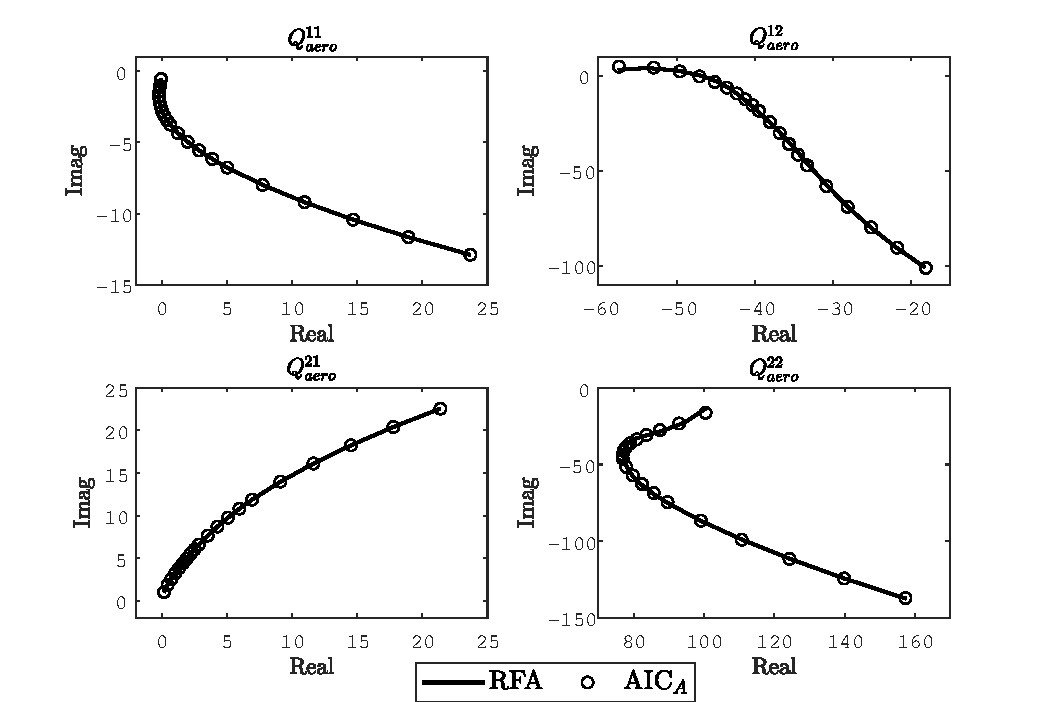
\includegraphics[width=\textwidth]{trabalho-graduacao/capitulos/figures/cap_4/RFAs/RFA_Modes.pdf}
    \label{fig:RFAsModes}
\end{figure}

\newpage

A aproximação dos termos aerodinâmicos referentes à superfície de controle, matriz $\boldsymbol{AIC}_{c}$, é apresentada na Figura \ref{fig:RFAsControl}. Destaca-se que os termos de aproximação também representam de forma apropriada o comportamento aerodinâmico não-estacionário para o movimento da superfície de controle.

\begin{figure}[ht!]
    \centering
    \caption{Comparação dos termos aerodinâmicos \gls{AICa} com a aproximação por \gls{RFA}}
    \noindent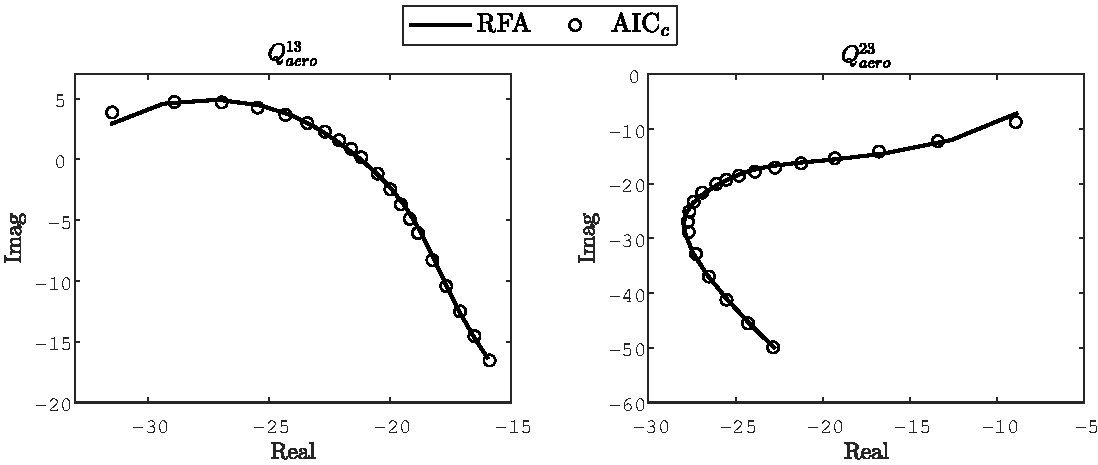
\includegraphics[width=\textwidth]{trabalho-graduacao/capitulos/figures/cap_4/RFAs/RFA_Control.pdf}
    \label{fig:RFAsControl}
\end{figure}
% ----------------------------------------------------------




% ----------------------------------------------------------
\section{Estabilidade em Malha Aberta}\label{sec:malha-aberta}

Após a determinação das matrizes de aproximação aerodinâmica, o modelo matemático no espaço de estados pode ser construído e a dinâmica do sistema avaliada. 

Inicialmente, um estudo da estabilidade em malha aberta do sistema foi realizado a partir do lugar geométrico das raízes para variação da velocidade do escoamento incidindo sobre a seção típica. Dessa forma, a velocidade de \textit{flutter} pode ser estimada como o valor na qual o lugar geométrico das raízes do sistema passe da região estável para a instável, isto é, do semiplano esquerdo para o direito do plano complexo.

Os resultado obtidos são apresentados na Figura \ref{fig:OpenLoop-Poles}, na qual pode ser observada a movimentação do conjunto de polos do sistema para diferentes velocidades. Destacada na figura está a velocidade de \textit{flutter}, como o ponto onde a parte real do respectivo polo é nula, representando a instabilidade do sistema para velocidades superiores à essa. Obteve-se o ponto de instabilidade do sistema como $V_{OLF} = 29,59$ m/s, corroborando o valor de velocidade de \textit{flutter} indicado por \textcite{book:Fung} para o respectivo modelo, com um erro inferior a $2\%$.

\begin{figure}[ht]
    \centering
    \caption{Lugar geométrico das raízes do sistema em malha aberta}
    \noindent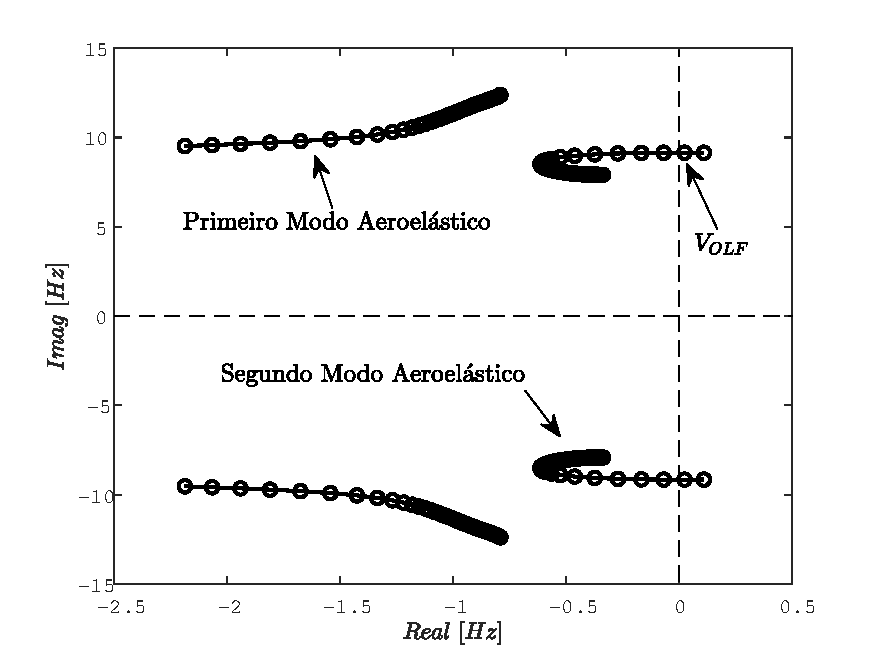
\includegraphics[width=\textwidth]{trabalho-graduacao/capitulos/figures/cap_4/Open-Loop/OpenLoop-Poles.pdf}
    \label{fig:OpenLoop-Poles}
\end{figure}

\newpage

Os polos referentes aos estados de atraso aerodinâmico foram omitidos devido ao desejo de destacar os polos que representam modos físicos do modelo, porém são apresentados na Tabela \ref{tab:VOLF-Poles}. As matrizes dinâmica, de entrada do sistema para a condição de \textit{flutter} em malha aberta, $V_{OLF} = 29,59$ m/s, foram obtidas como

\[
\boldsymbol{A} = 
\begin{bmatrix}
	\boldsymbol{0}_{2 \times 2} & \boldsymbol{I}_{2 \times 2}   & \boldsymbol{0}_{2 \times 8}   & \boldsymbol{0}_{2 \times 3} 	\\
	\boldsymbol{A}_{1} 	        & \boldsymbol{A}_{2} 	        & \boldsymbol{A}_{3} 	        & \boldsymbol{A}_{4} 		    \\
	\boldsymbol{0}_{8 \times 2} & \boldsymbol{A}_{5}  	        & \boldsymbol{A}_{6}	        & \boldsymbol{A}_{7}		    \\
	\boldsymbol{0}_{3 \times 2} & \boldsymbol{0}_{3 \times 2}   & \boldsymbol{0}_{2 \times 8}   & \boldsymbol{A}_{8}		    \\
\end{bmatrix}, \ \boldsymbol{B} = \begin{bmatrix}  \boldsymbol{0}_{14 \times 1} \\ 6,697\cdot10^{6} \end{bmatrix}
\]

\noindent onde as matrizes $\boldsymbol{A}_{i}$, sendo $i=1, 2, \cdots, 8$, que definem a matriz dinâmica $\boldsymbol{A}$ são dadas por

\[
\boldsymbol{A}_{1} = 
\begin{bmatrix}
-3682,960 & -3635,719 \\
476,618 & -2410,689
\end{bmatrix}, \ 
\boldsymbol{A}_{2} = 
\begin{bmatrix}
-11,014 & -14,789 \\
1,976 & -7,860
\end{bmatrix}
\]

\[
\boldsymbol{A}_{3} = 
\begin{bmatrix}
    133,688 & -17,283 & 133,688 & -17,283 & 133,688 & -17,283 & 133,688 & -17,283 \\
    -17,277 & 13,895 & -17,277 & 13,895 & -17,277 & 13,895 & -17,277 & 13,895
\end{bmatrix}
\]

\[
\boldsymbol{A}_{4} = 
\begin{bmatrix}
    -4,676 & -191,056 & 0,062 \\
    0,512 & -48,397 & 0,071
\end{bmatrix}, \
\boldsymbol{A}_{5} = 
\begin{bmatrix} 
    0,834 & 36,040      \\
    1,459 & -63,069     \\
    0,382 & -62,820     \\
    0,668 & 109,935     \\
    -1,085 & 94,801     \\
    1,898 & -165,902    \\
    0,073 & -47,649     \\
    0,128 & 83,387      \\
\end{bmatrix}
\]

\[
diag\left( \begin{bmatrix} -46,6 & -46,6 & -93,2 & -93,2 & -139,8 & -139,8 & -186,4 & -186,4 \end{bmatrix} \right)
\]

\[
\boldsymbol{A}_{7} = 
\begin{bmatrix}
    0 & 20,685  &  0 \\
    0 & -36,198 &  0 \\
    0 & -34,938 &  0 \\
    0 & 61,141  &  0 \\
    0 & 53,255  &  0 \\
    0 & -93,196 &  0 \\
    0 & -26,274 &  0 \\
    0 & 45,980  &  0 \\
\end{bmatrix}, \ 
\boldsymbol{A}_{8} = 
\begin{bmatrix}
    0 & 1 & 0 \\
    0 & 0 & 1 \\
    -6,697\cdot10^{6} & -5,330\cdot10^{4} & -2,827\cdot10^{2}
\end{bmatrix}
\]

\begin{table}[h]
\centering
\caption{Polos do sistema em malha aberta para velocidade $V_{OLF} = 29,59$ m/s}
\begin{tabular}{ccc} 
Polo em malha fechada & Valor do polo & Relação com variável de estado \\ \hline
$p_{1} $  & $0+0,575i$ & primeiro \gls{GDL}, $h$                                \\
$p_{2} $  & $0-0,575i$ & primeiro \gls{GDL}, $h$                                \\
$p_{3} $  & $-0,128+0,603i$ & segundo \gls{GDL}, $\theta$                       \\
$p_{4} $  & $-0,128-0,603i$ & segundo \gls{GDL}, $\theta$                       \\
$p_{5} $  & $-1,941+0i$ &  atraso aerodinâmico devido à \gls{RFA}          \\
$p_{6} $  & $-1,142+0,176i$ & atraso aerodinâmico devido à \gls{RFA}       \\
$p_{7} $  & $-1,142-0,176i$ & atraso aerodinâmico devido à \gls{RFA}       \\
$p_{8} $  & $-0,370+0i$ & atraso aerodinâmico devido à \gls{RFA}           \\
$p_{9} $  & $-1,864+0i$ & atraso aerodinâmico devido à \gls{RFA}           \\
$p_{10} $ & $-1,398+0i$ & atraso aerodinâmico devido à \gls{RFA}           \\
$p_{11} $ & $-0,932+0i$ & atraso aerodinâmico devido à \gls{RFA}           \\
$p_{12} $ & $-0,466+0i$ & atraso aerodinâmico devido à \gls{RFA}           \\
$p_{13} $ & $-1,885+0i$ & movimento da superfície de controle                   \\
$p_{14} $ & $-0,471+1,825i$ & movimento da superfície de controle               \\
$p_{15} $ & $-0,4712-1,825i$ & movimento da superfície de controle              \\
\hline
\end{tabular}
\label{tab:VOLF-Poles}
\end{table}

\newpage

Na Figura \ref{fig:OpenLoopSimulation}, é apresentada a resposta dinâmica do sistema no domínio do tempo, obtidos a partir de simulações numéricas em malha aberta, para uma condição inicial de $0,127$ m no primeiro grau de liberdade. A condição inicial imposta emula uma perturbação vista pelo sistema em relação à sua condição de equilíbrio e seu valor foi definido igual o parâmetro de meia corda do sistema.

Como esperado, para a condição de velocidade igual à velocidade de \textit{flutter} resultante da análise de estabilidade, a resposta dinâmica do sistema não mostra amortecimento da vibração estrutural. O resultado de simulação numérica alinhado com a análise de estabilidade em malha aberta a capacidade do modelo numérico desenvolvido de capturar a dinâmica do sistema não somente para movimentos oscilatórios desenvolvidos, mas garantindo representatividade na região transiente, como nos primeiros instantes de simulação apresentados na figura acima.

\begin{figure}[ht]
    \centering
    \caption{Simulação em malha aberta, para uma velocidade $V_{\infty} = 29,59$ m/s}
    \noindent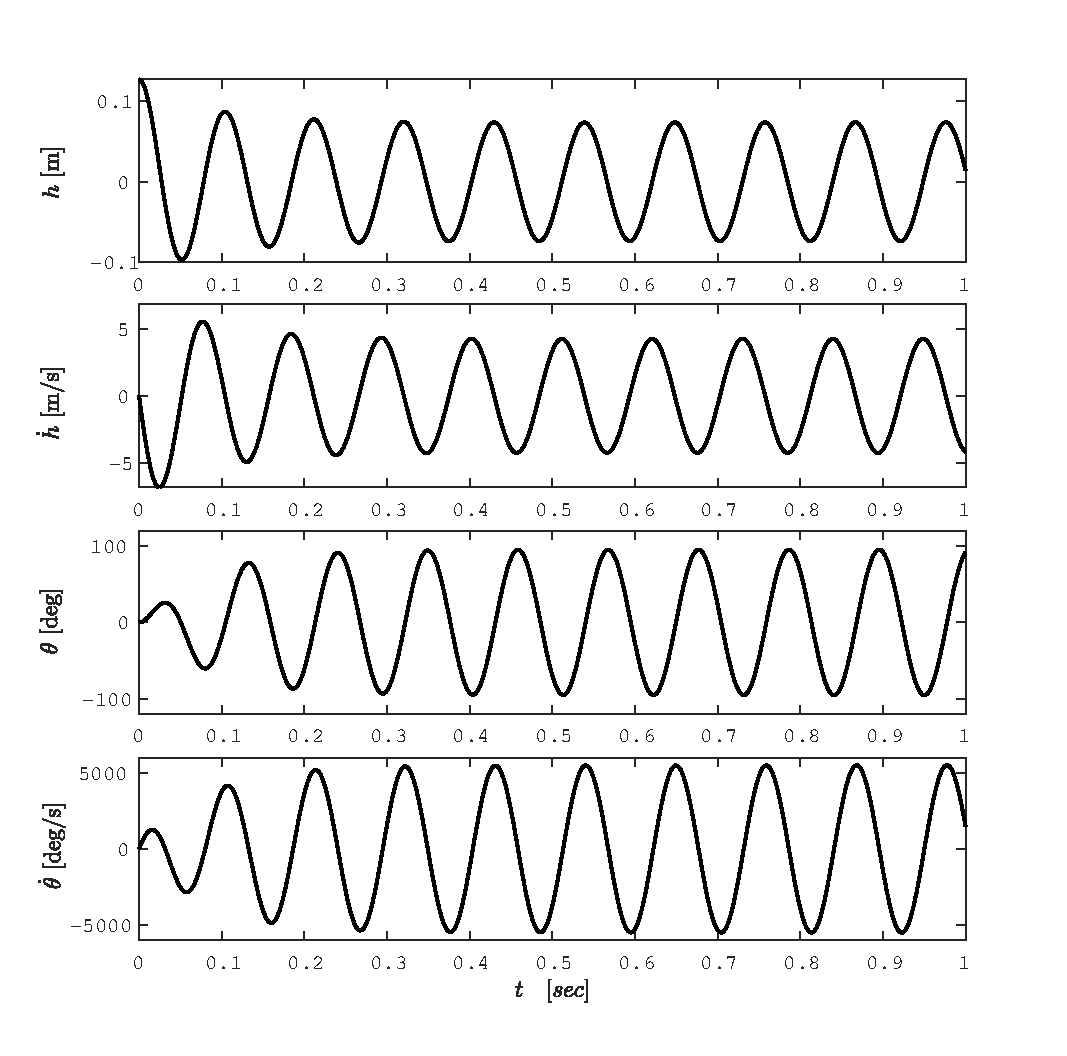
\includegraphics[width=0.95\textwidth]{trabalho-graduacao/capitulos/figures/cap_4/Open-Loop/OpenLoop-Simulation.pdf}
    \label{fig:OpenLoopSimulation}
\end{figure}


% ----------------------------------------------------------

% ----------------------------------------------------------
\section{Resultados em malha fechada}\label{sec:malha-fechada}

O modelo matemático calculado para a condição de $V_{OLF}$ foi utilizado para o desenvolvimento da lei de controle por realimentação de estados.

Para isso, inicialmente realizou-se a discretização do modelo para contabilizar os efeitos de amostragem no projeto da lei de controle. Adotou-se um período de amostragem igual à $0,01$ s, obtendo-se as matrizes do sistema digital como

\[
    \boldsymbol{\Phi} = \begin{bmatrix}
        \boldsymbol{\phi}_{1} & \boldsymbol{\phi}_{2} & \boldsymbol{\phi}_{3} \\
        \boldsymbol{\phi}_{4} & \boldsymbol{\phi}_{5} & \boldsymbol{\phi}_{6} \\
        \boldsymbol{\phi}_{7} & \boldsymbol{\phi}_{8} & \boldsymbol{\phi}_{9}
    \end{bmatrix}, \quad
    \boldsymbol{\Gamma} = \begin{bmatrix}  
    -0,288 \\ -0,105 \\ -88,008 \\ -30,247 \\ 5,542 \\ -9,699 \\ 
    -7,728 \\ 13,523 \\ 10,486 \\ -18,351 \\ -4,418 \\ 7,731  \\ 
    0,483 \\ 97,622 \\ 3,768\cdot10^{3}  
    \end{bmatrix}
\]

\noindent sendo as matrizes $\boldsymbol{\phi}_{i}$, para $i=1,2,\cdots,9$, definidas para melhor visualização como

\[
\boldsymbol{\phi}_{1} = 
\begin{bmatrix}
    0,827   & 0,164     & 0,009     & 0,001     & 0,005 \\
    0,021   & 0,884     & 0         & 0,009     & 0,001 \\
   -32,985  & -30,453   & 0,719     & 0,146     & 0,946 \\
    3,721   & -22,557   & 0,039     & 0,775     & 0,105 \\
    0,762   & -3,481    & 0,001     & 0,260     & 0,604 \\
\end{bmatrix}
\]

\[
\boldsymbol{\phi}_{2} = 
\begin{bmatrix}
    0,001 & 0,005 & 0,001 & 0,004 & 0,001 \\
    0,001 & 0,001 & 0     & 0     & 0     \\
    0,130 & 0,761 & 0,105 & 0,623 & 0,086 \\
    0,098 & 0,083 & 0,078 & 0,067 & 0,064 \\
    0,018 & 0,020 & 0,015 & 0,018 & 0,013 \\
\end{bmatrix}, \ 
\boldsymbol{\phi}_{3} = 
\begin{bmatrix}
    0,004 & 0      &  0,288 & 0,006 & 0      \\
    0     & 0      &  0,105 & 0,001 & 0      \\
    0,518 & 0,072  & 87,966 & 0,582 & 0,002  \\
    0,055 &  0,053 & 30,251 & 0,148 & 0,001  \\
    0,015 &  0,012 & -5,541 &  0,031 &  0    \\
\end{bmatrix}
\]


\[
\boldsymbol{\phi}_{4} = 
\begin{bmatrix}
   -1,334 &  6,092 &  0,001 & 0,455 &  0,041 \\
   -1,012 &  5,406 & 0,006 & 0,365 &  0,031 \\
    1,772 & -9,461 &  0,010 &  0,639 & 0,054 \\
    1,394 & -7,114 &  0,006 &  0,452 & 0,042 \\
   -2,440 & 12,450 & 0,010 & 0,791 &  0,074
\end{bmatrix}
\]

\[
\boldsymbol{\phi}_{5} = 
\begin{bmatrix}
 0,597 &  0,035 & 0,027 &  0,031 & 0,023 \\
 0,026 &  0,420 & 0,022 &  0,023 & 0,019 \\
 0,046 & 0,046 &  0,433 & 0,040 &  0,034 \\
 0,035 & 0,036 &  0,029 &  0,216 &  0,025 \\
 0,060 &  0,063 & 0,052 &  0,054 &  0,202
\end{bmatrix}, \ 
\boldsymbol{\phi}_{6} = 
\begin{bmatrix}
 0,027 & 0,021 &  9,698 & 0,055 & 0       \\
 0,020 & 0,017 &  7,726 & 0,023 & 0       \\
 0,035 &  0,030 & -13,521 & 0,041 &  0    \\
 0,027 &  0,022 & -10,485 & 0,015 &  0    \\
 0,047 & 0,039 & 18,349 & 0,026 & 0
\end{bmatrix}
\]


\[
\boldsymbol{\phi}_{7} = 
\begin{bmatrix}
    0,572 &  3,217 & 0,005 & 0,189 & 0,017 \\
    1,001 & -5,630 & 0,008 & 0,331 & 0,030 \\
    0 &  0 &  0 &  0 &  0 \\
    0 &  0 &  0 &  0 &  0 \\
    0 &  0 &  0 &  0 &  0
\end{bmatrix}\]

\[ 
\boldsymbol{\phi}_{8} = 
\begin{bmatrix}
 0,015 &  0,015 & 0,013 & 0,013 & 0,011 \\
 0,026 & 0,026 &  0,022 & 0,022 & 0,019 \\
 0 &  0 &  0 &  0 &  0 \\
 0 &  0 &  0 &  0 &  0 \\
 0 &  0 &  0 &  0 &  0 
\end{bmatrix}
\]

\[
\boldsymbol{\phi}_{9} = 
\begin{bmatrix}
 0,166 & 0,010 &  4,417 &  0,002 & 0         \\
 0,019 &  0,172 & -7,730 & 0,004 &  0      \\
 0 &  0 &  0,517 &  0,005 &  0             \\
 0 &  0 & -97,622 & 0,260 &  0,001         \\
 0 &  0 & -3768,616 & -127,611 & 0,419
\end{bmatrix}
\]


Para projetar a lei de controle, definiram-se os pesos como

\[    
\boldsymbol{W}_{x} = 1\cdot10^{3}\boldsymbol{I}_{N_{x}};  \quad \boldsymbol{W}_{u} = 1
\]

O problema do \gls{LQR} foi resolvido utilizando o \textit{software} MatLab, encontrando-se

\[
\begin{split}
\boldsymbol{K} &= 
[\begin{matrix} 1,942 &  8,956 & -0,070 & -0,027 & -0,116 & -0,005 & -0,088 &  0,001 & -0,064 \end{matrix} \\
&\qquad\qquad\qquad\qquad \begin{matrix} 0,002 & -0,049 &  0,002 & -999,877 & -9,283 & -0,019 \end{matrix}]
\end{split}
\]

Além de resultados de simulação, avaliou-se a evolução dos polos de malha fechada para variações na velocidade de \textit{flutter} utilizando o lugar geométrico das raízes (vide Figura \ref{fig:ClosedLoop-Poles}). Como pode ser observado, o controlador garante a estabilização do sistema na condição de $V_{OLF}$, condição de projeto da lei de controle. Mais ainda, a estabilidade é mantida até $\gls{VCLF}=31,37$ m/s. Apesar do aumento em $6 \%$ da velocidade de \textit{flutter} do sistema em malha fechada quando comparado à original, a introdução da estrutura de controle para supressão de \textit{flutter} não apresenta garantia de estabilidade para velocidades acima da de projeto, sendo esse aumento percentual uma consequência sem garantia teórica.

Para estabilizar o sistema na nova velocidade de flutter $\gls{VCLF}$, um novo modelo no espaço de estados deve ser calculado, o que torna necessário recalcular as matrizes de aproximação aerodinâmica. De posse do novo modelo, projeta-se um novo controlador por realimentação de estados. Então, durante a operação,  chaveia-se para o novo vetor de realimentação de estados quando o sistema estiver suficientemente próximo de tal velocidade. Alternativamente uma abordagem de escalonamento de ganhos poderia ser adotada para suavizar a transição entre diferentes pontos de operação.

Os valor dos polos em malha fechada para a velocidade $\gls{VCLF}$ são apresentados na Tabela \ref{tab:VOLF-ClosedLoop-Poles}.

\begin{table}[h]
\centering
\caption{Polos do sistema discreto em malha fechada para velocidade de \textit{flutter} em malha aberta ($V_{OLF} = 29,59$ m/s)}
\begin{tabular}{ccc} 
Polo em malha fechada & Valor do polo & Relação com variável de estado \\ \hline
$p_{1} $  & $0,822 + 0,532i$ & primeiro \gls{GDL}, $h$                  \\
$p_{2} $  & $0,822 - 0,532i$ & primeiro \gls{GDL}, $h$                  \\
$p_{3} $  & $0,725 + 0,499i$ & segundo \gls{GDL}, $\theta$              \\
$p_{4} $  & $0,725 - 0,499i$ & segundo \gls{GDL}, $\theta$              \\
$p_{5} $  & $1 + 0i$ &  atraso aerodinâmico devido à \gls{RFA}          \\
$p_{6} $  & $0,314 + 0,056i$ & atraso aerodinâmico devido à \gls{RFA}   \\
$p_{7} $  & $0,314 - 0,056i$ & atraso aerodinâmico devido à \gls{RFA}   \\
$p_{8} $  & $0,6910 + 0i$ & atraso aerodinâmico devido à \gls{RFA}      \\
$p_{9} $  & $0,0000 + 0i$ & atraso aerodinâmico devido à \gls{RFA}      \\
$p_{10} $ & $0,329 + 0i$ & atraso aerodinâmico devido à \gls{RFA}       \\
$p_{11} $ & $0,1436 + 0i$ & atraso aerodinâmico devido à \gls{RFA}      \\
$p_{12} $ & $0,6275 + 0i$ & atraso aerodinâmico devido à \gls{RFA}      \\
$p_{13} $ & $0,3938 + 0i$ & movimento da superfície de controle         \\
$p_{14} $ & $0,1551 + 0i$ & movimento da superfície de controle         \\
$p_{15} $ & $0,2471 + 0i$ & movimento da superfície de controle         \\
\hline
\end{tabular}
\label{tab:VOLF-ClosedLoop-Poles}
\end{table}

\begin{figure}[ht!]
    \centering
    \caption{Lugar geométrico das raízes discreto em malha fechada para diferentes velocidades}
    \noindent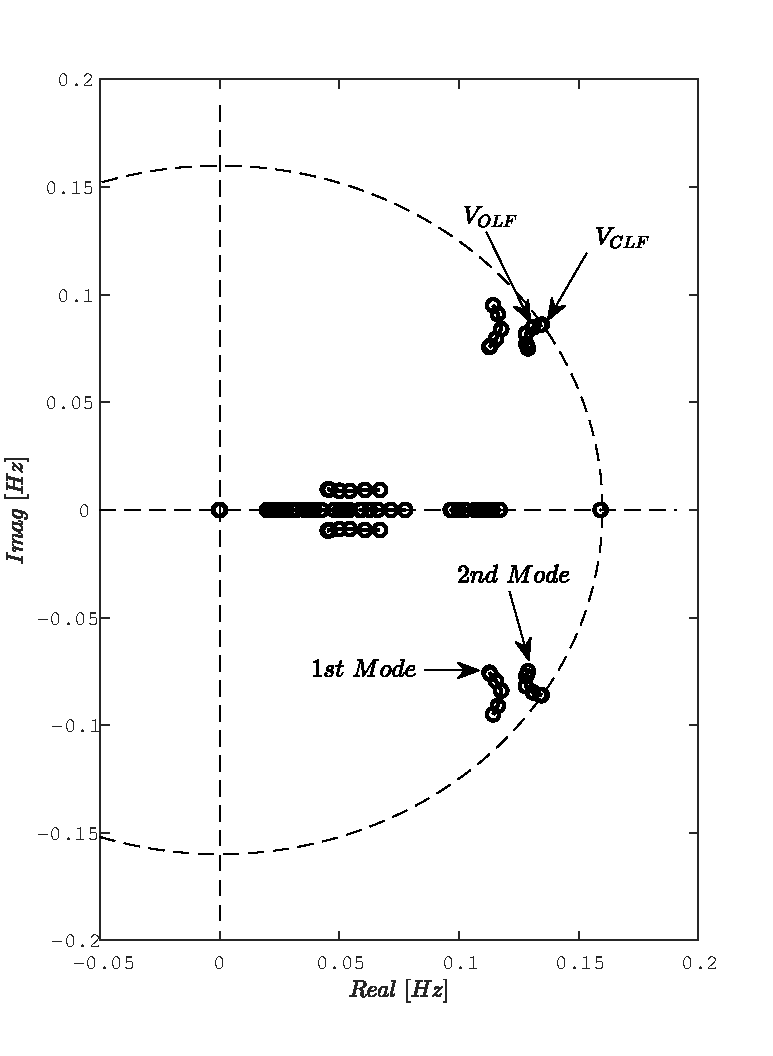
\includegraphics[width=\textwidth]{trabalho-graduacao/capitulos/figures/cap_4/Closed-Loop-Poles/ClosedLoopPoles.pdf}

    \label{fig:ClosedLoop-Poles}
\end{figure}

A avaliação do comportamento dinâmico do sistema em malha fechada também foi realizada a partir de simulações numéricas computacionais. Foram estudadas distintas condições de voo, para velocidades menores, igual e maiores à $V_{OLF}$, todas para condição ISA no nível do mar. As simulações foram realizadas utilizando-se condições iniciais impostas ao primeiro estado, referente ao deslocamento primeiro \gls{GDL}, $h$, emulando uma perturbação em relação à condição de equilíbrio.

\newpage

A Figura \ref{fig:CloseLoopResponse-t0-VOLF} mostra a resposta dinâmica dos \gls{GDL}s do sistema para uma simulação realizada na condição de $V_{OLF}$, para condição inicial $h = 0,127$ m no sistema. Percebe-se que, com a ação do controlador projetado, o sistema é capaz de eliminar a oscilação de \textit{flutter} em malha aberta, cumprindo a regulação do sistema. 

\begin{figure}[ht!]
    \centering
    \caption{Resposta dinâmica em malha fechada, para uma velocidade $V_{\infty} = 29,59$ m/s, com condição inicial não nula no primeiro \gls{GDL} igual à $h=0,127$ m}
    \noindent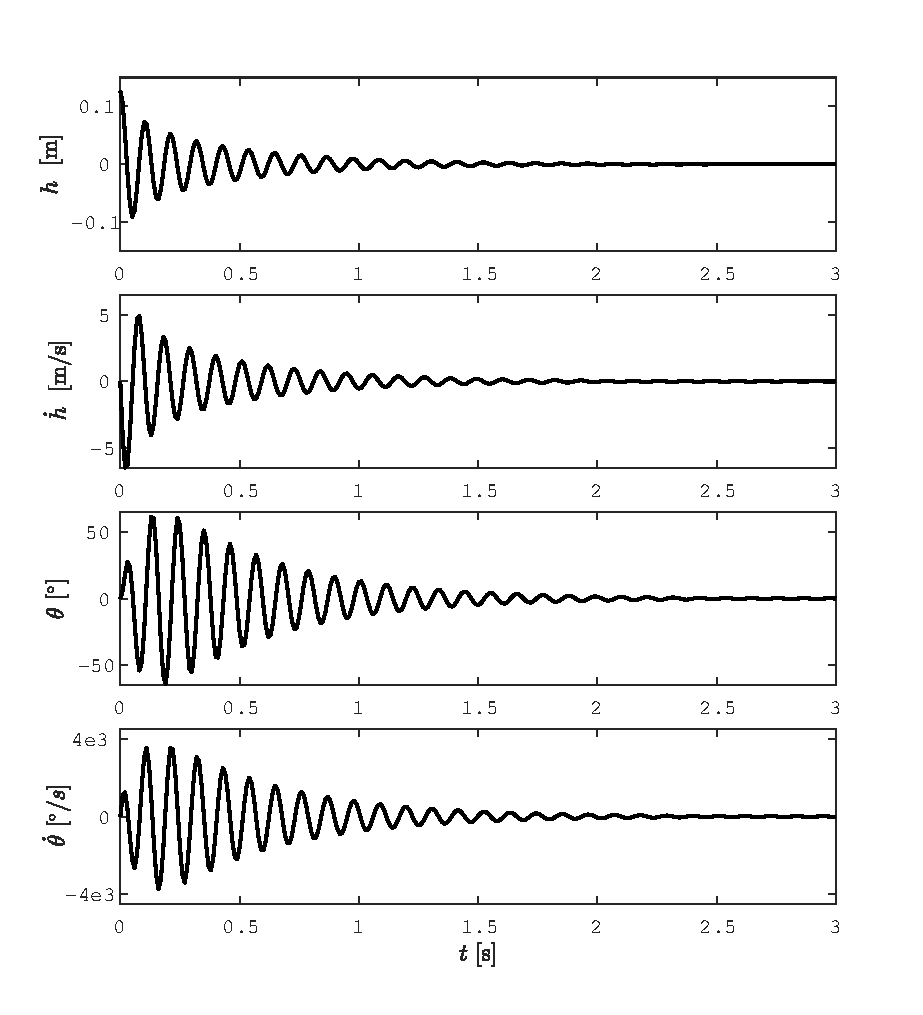
\includegraphics[width=\textwidth]{trabalho-graduacao/capitulos/figures/cap_4/Closed-Loop-Simulation/CLSimulation-VOLF-t0-modes.pdf}
    \label{fig:CloseLoopResponse-t0-VOLF}
\end{figure}


A ação de controle calculada a cada instante de tempo é apresentada na Figura \ref{fig:CloseLoopControl-t0-VOLF}, junto dos estados referentes ao movimento da superfície de controle. Avaliando os resultados, destaca-se o atraso do movimento angular da superfície em relação à entrada calculada pelo controlador, proveniente da dinâmica do atuador. Percebe-se, também, que o sistema apresenta um erro em regime permanente, sendo o a deflexão da superfície de controle não retornando à sua posição inicial, e o sistema assumindo uma nova posição de equilíbrio aeroelástico estático. Como discutido por \textcite{art:Sun-2014}, isso é resultado da não controlabilidade do sistema, conforme apresentado na seção anterior.


\begin{figure}[ht!]
    \centering
    \caption{Ação de controle e estados da superfície de controle, para uma velocidade $V_{\infty} = 29,59$ m/s, com condição inicial não nula no primeiro \gls{GDL} igual à $h=0,127$ m}
    \noindent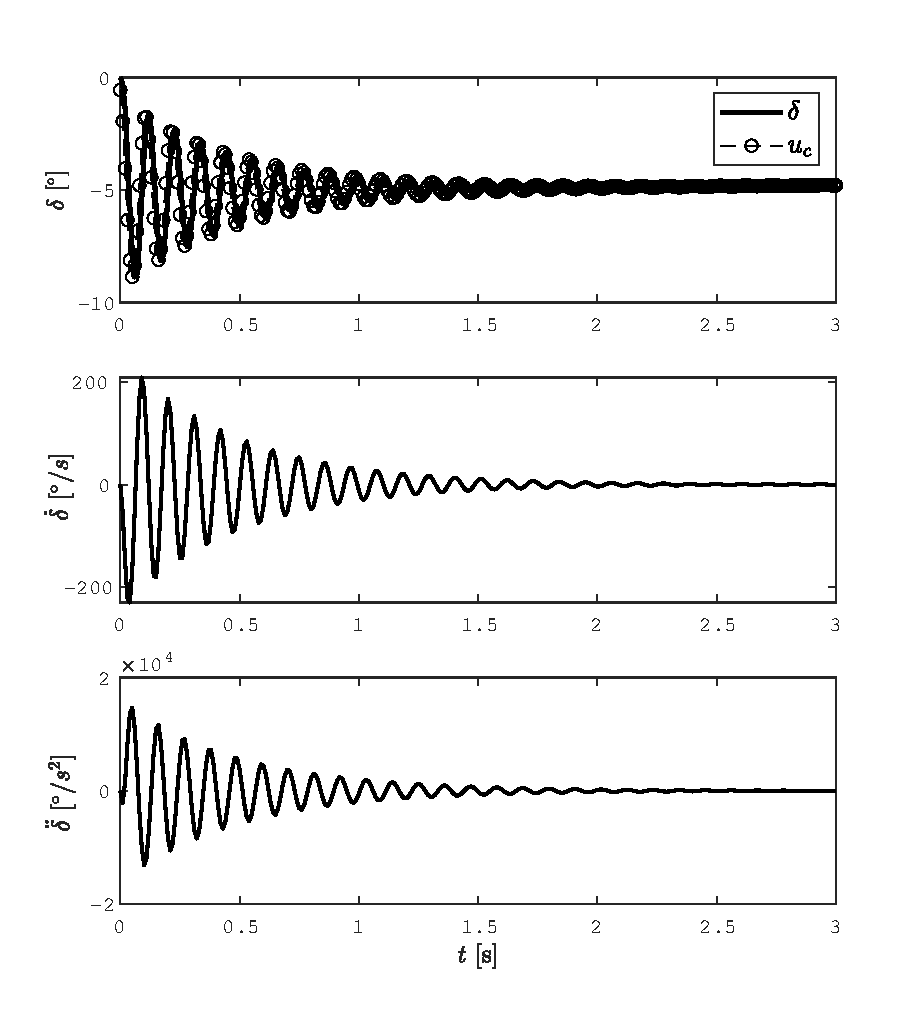
\includegraphics[width=\textwidth]{trabalho-graduacao/capitulos/figures/cap_4/Closed-Loop-Simulation/CLSimulation-VOLF-t0-control.pdf}
    \label{fig:CloseLoopControl-t0-VOLF}
\end{figure}

\newpage
O novo ponto de instabilidade do sistema em malha fechada, $\gls{VCLF}$, também foi avaliado em simulação com uma perturbação no estado inicial. Os resultados são mostrados nas Figuras \ref{fig:CloseLoopResponse-t0-VCLF} e \ref{fig:CloseLoopControl-t0-VCLF}. Apesar da ação do controlador sobre o sistema evitar que a resposta dinâmica divirja, para essa velocidade do escoamento, a estrutura de controle também não é capaz de estabilizar o movimento.

\begin{figure}[ht!]
    \centering
    \caption{Resposta dinâmica em malha fechada, para uma velocidade $V_{\infty} = 31,37$ m/s, com condição inicial não nula no primeiro \gls{GDL} igual à $h=0,127$ m}
    \noindent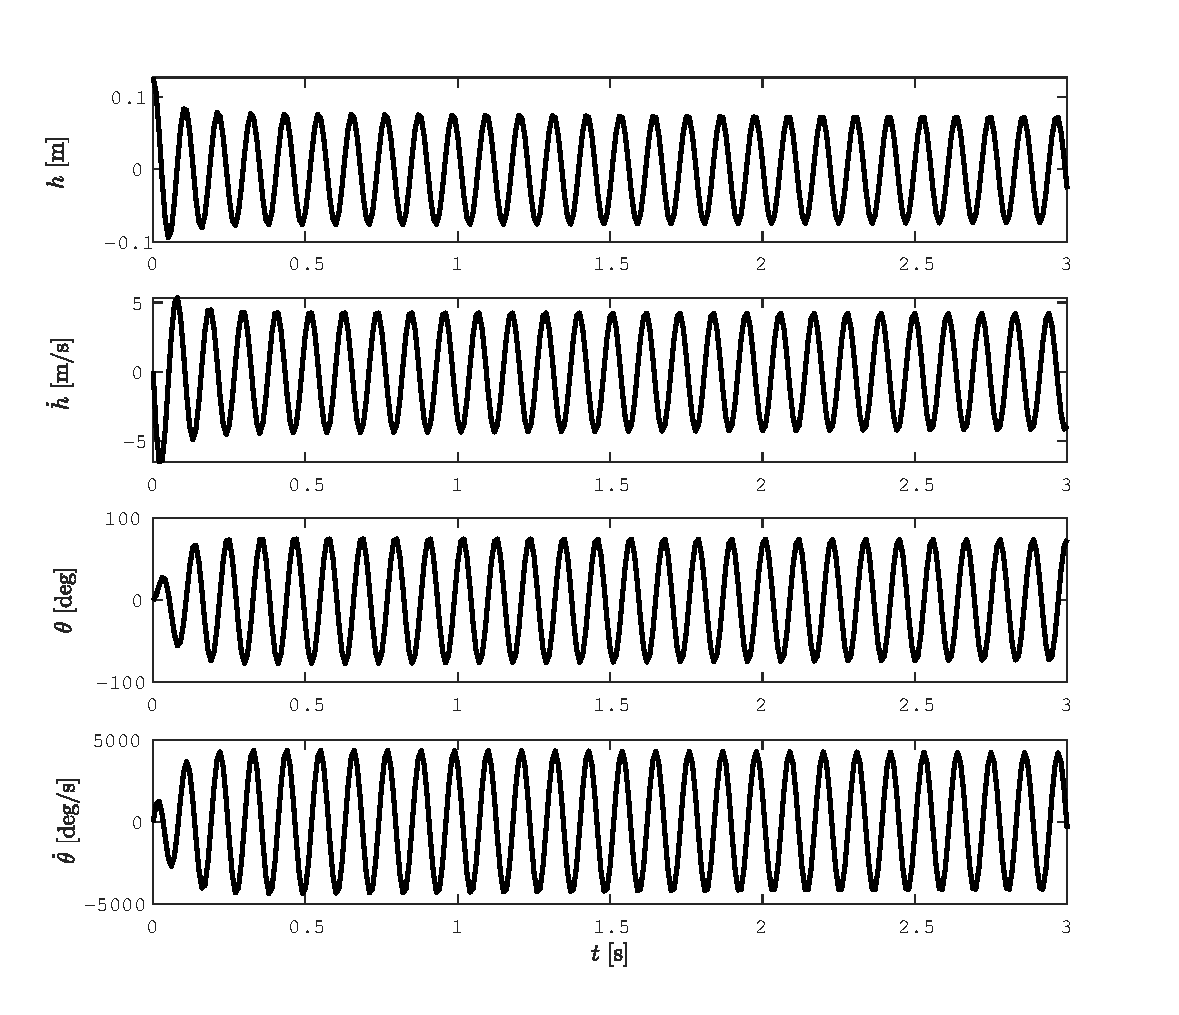
\includegraphics[width=\textwidth]{trabalho-graduacao/capitulos/figures/cap_4/Closed-Loop-Simulation/CLSimulation-VCLF-t0-modes.pdf}

    \label{fig:CloseLoopResponse-t0-VCLF}
\end{figure}

\begin{figure}[ht!]
    \centering
    \caption{Ação de controle e estados da superfície de controle, para uma velocidade $V_{\infty} = 31,37$ m/s, com condição inicial não nula no primeiro \gls{GDL} igual à $h=0,127$ m}
    \noindent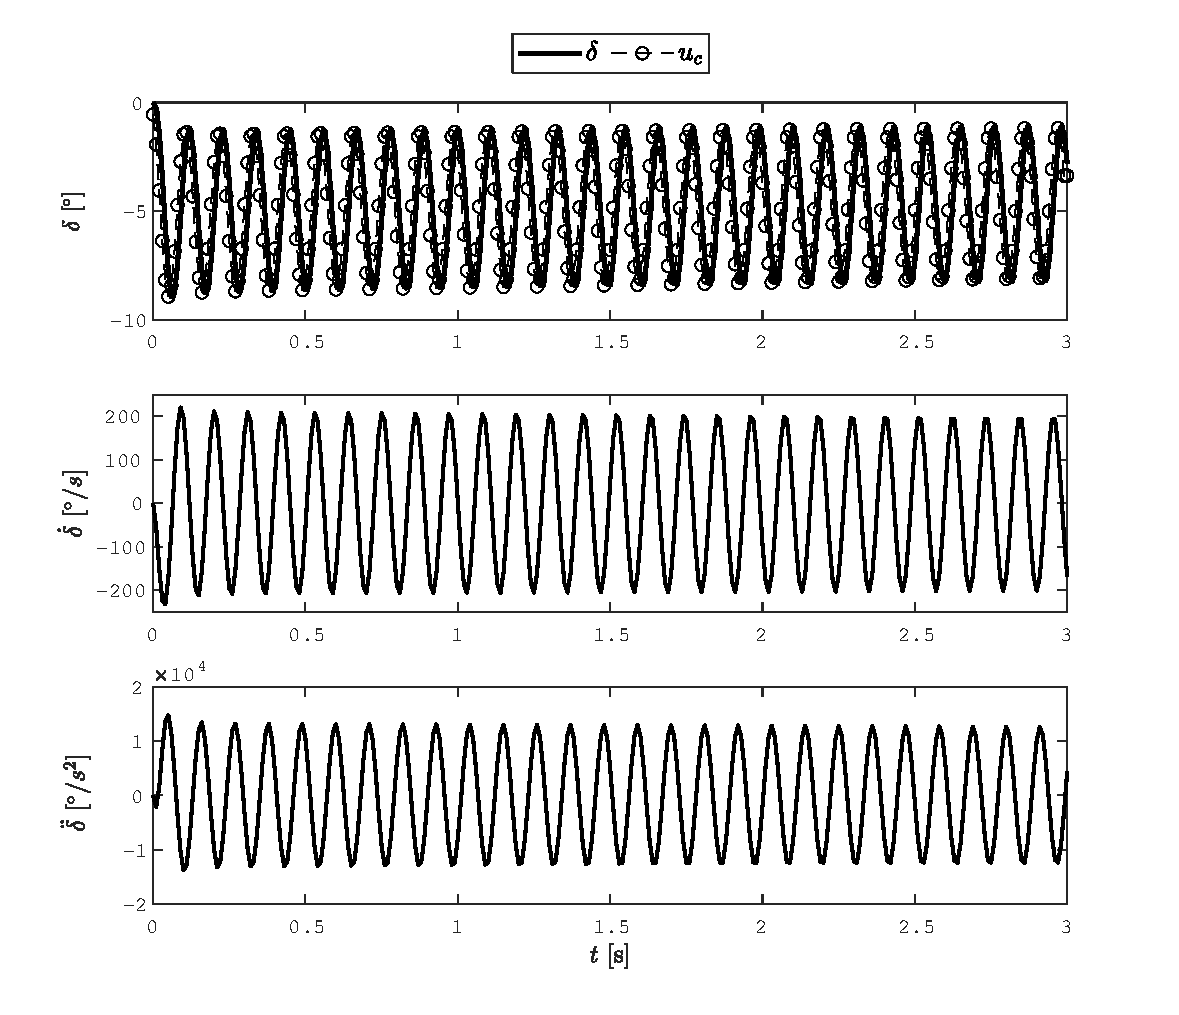
\includegraphics[width=\textwidth]{trabalho-graduacao/capitulos/figures/cap_4/Closed-Loop-Simulation/CLSimulation-VCLF-t0-control.pdf}
    \label{fig:CloseLoopControl-t0-VCLF}
\end{figure}

Avaliou-se também, o efeito da lei de controle implementada em velocidades inferiores à de instabilidade em malha aberta, $V_{OLF}$. Conforme apresentado na Figura \ref{fig:CloseLoopResponse-t0-1000}, a estrutura em malha fechada para o sistema é capaz de reduzir o tempo necessário para os \gls{GDL}s retornarem à posição de equilíbrio. Entretanto, identificou-se que, para velocidades inferiores à $2,50$ m/s, a presença do controlador projetado para a condição de $V_{OLF}$ desestabilizou o sistema, como mostrado pelos resultados de simulação das Figuras \ref{fig:CloseLoopResponse-t0-VLVF} e \ref{fig:CloseLoopControl-t0-VLVF}. Essa característica é explicada pela operação muito longe da condição de projeto do controlador, alinhada ao sistema ser não controlável, resultando na não garantia da robustez da resposta em malha fechada para condições fora da região de projeto. Para referência, são apresentados na Figura \ref{fig:CloseLoopPoles} os polos do sistema em malha fechada para essa condição de instabilidade em velocidades baixas em malha fechada, denominada $\gls{VLVI}$. Percebe-se que os polos referentes aos primeiros modos do sistema, associados aos graus de liberdade da seção típica, estão contidos no círculo unitário, portanto são estáveis para essa condição. O polo instável é dado para frequência nula, e analisando esse dado junto do resultado de simulação podemos concluir que está associado ao movimento da superfície de controle.

\begin{figure}[ht]
    \centering
    \caption{Resposta dinâmica em malha fechada, para uma velocidade $V_{\infty} = 25,0$ m/s, com condição inicial não nula no primeiro \gls{GDL} igual à $h=0,127$ m}
    \noindent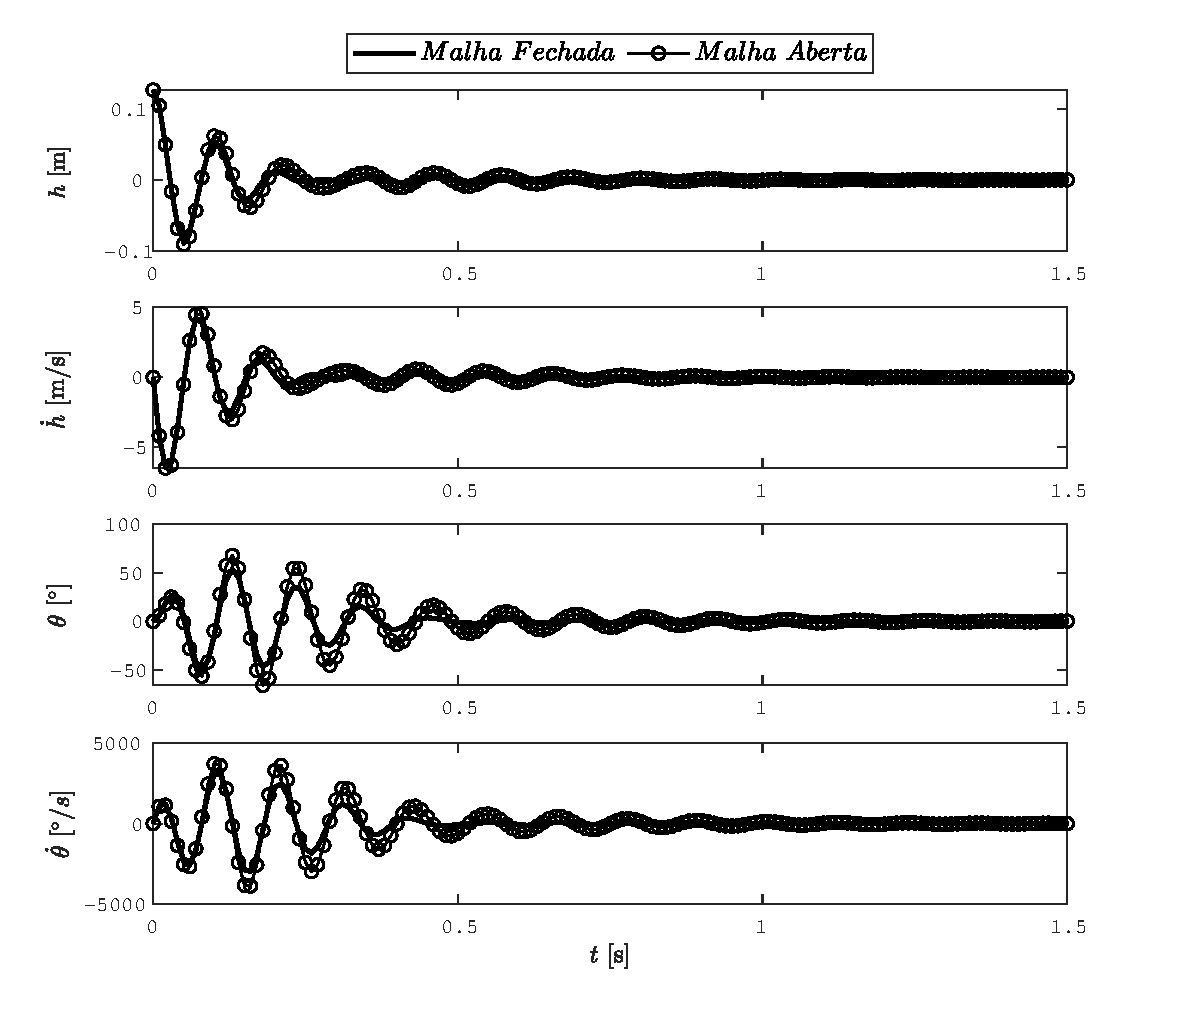
\includegraphics[width=\textwidth]{trabalho-graduacao/capitulos/figures/cap_4/Closed-Loop-Simulation/CLSimulation-1000-t0-modes.pdf}
    \label{fig:CloseLoopResponse-t0-1000}
\end{figure}

Por essa instabilidade estar associada à uma frequência nula, ela é definida como do tipo divergência dinâmica e não \textit{flutter}, como definido por \textcite{book:Wright-Cooper}.

\begin{figure}[ht]
    \centering
    \caption{Resposta dinâmica em malha fechada, para uma velocidade $V_{\infty} = 2,50$ m/s $(\gls{VLVI})$, com condição inicial não nula no primeiro \gls{GDL} igual à $h=0,127$ m}
    \noindent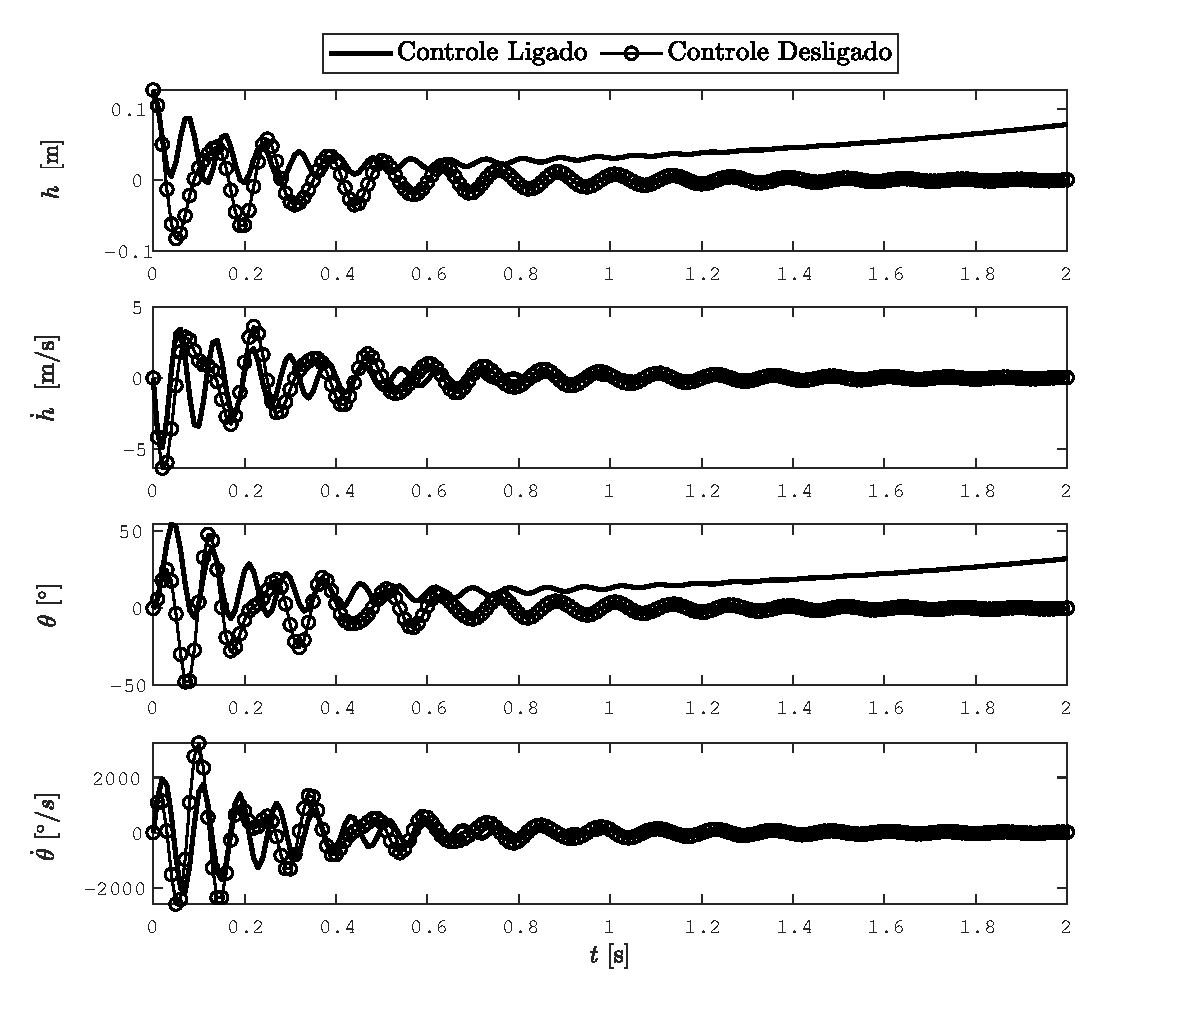
\includegraphics[width=\textwidth]{trabalho-graduacao/capitulos/figures/cap_4/Closed-Loop-Simulation/CLSimulation-VLVF-t0-modes.pdf}
    \label{fig:CloseLoopResponse-t0-VLVF}
\end{figure}

\begin{figure}[ht]
    \centering
    \caption{Ação de controle e estados da superfície de controle, para uma velocidade $V_{\infty} = 2,50$ m/s $(\gls{VLVI})$, com condição inicial não nula no primeiro \gls{GDL} igual à $h=0,127$ m}
    \noindent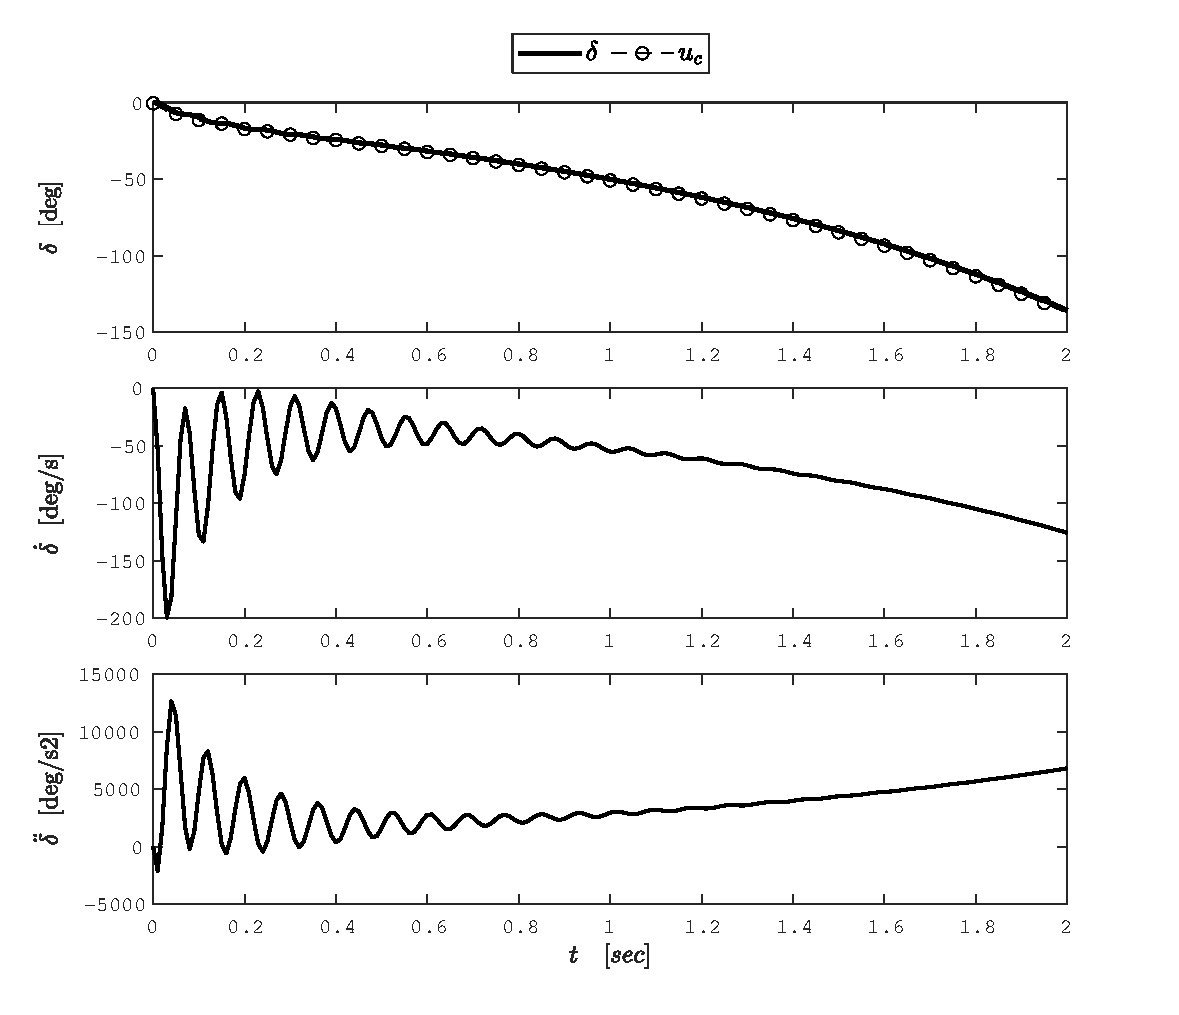
\includegraphics[width=\textwidth]{trabalho-graduacao/capitulos/figures/cap_4/Closed-Loop-Simulation/CLSimulation-VLVF-t0-control.pdf}
    \label{fig:CloseLoopControl-t0-VLVF}
\end{figure}

\begin{figure}[ht]
    \centering
    \caption{Polos em malha fechada para condição $\gls{VLVI}$}
    \noindent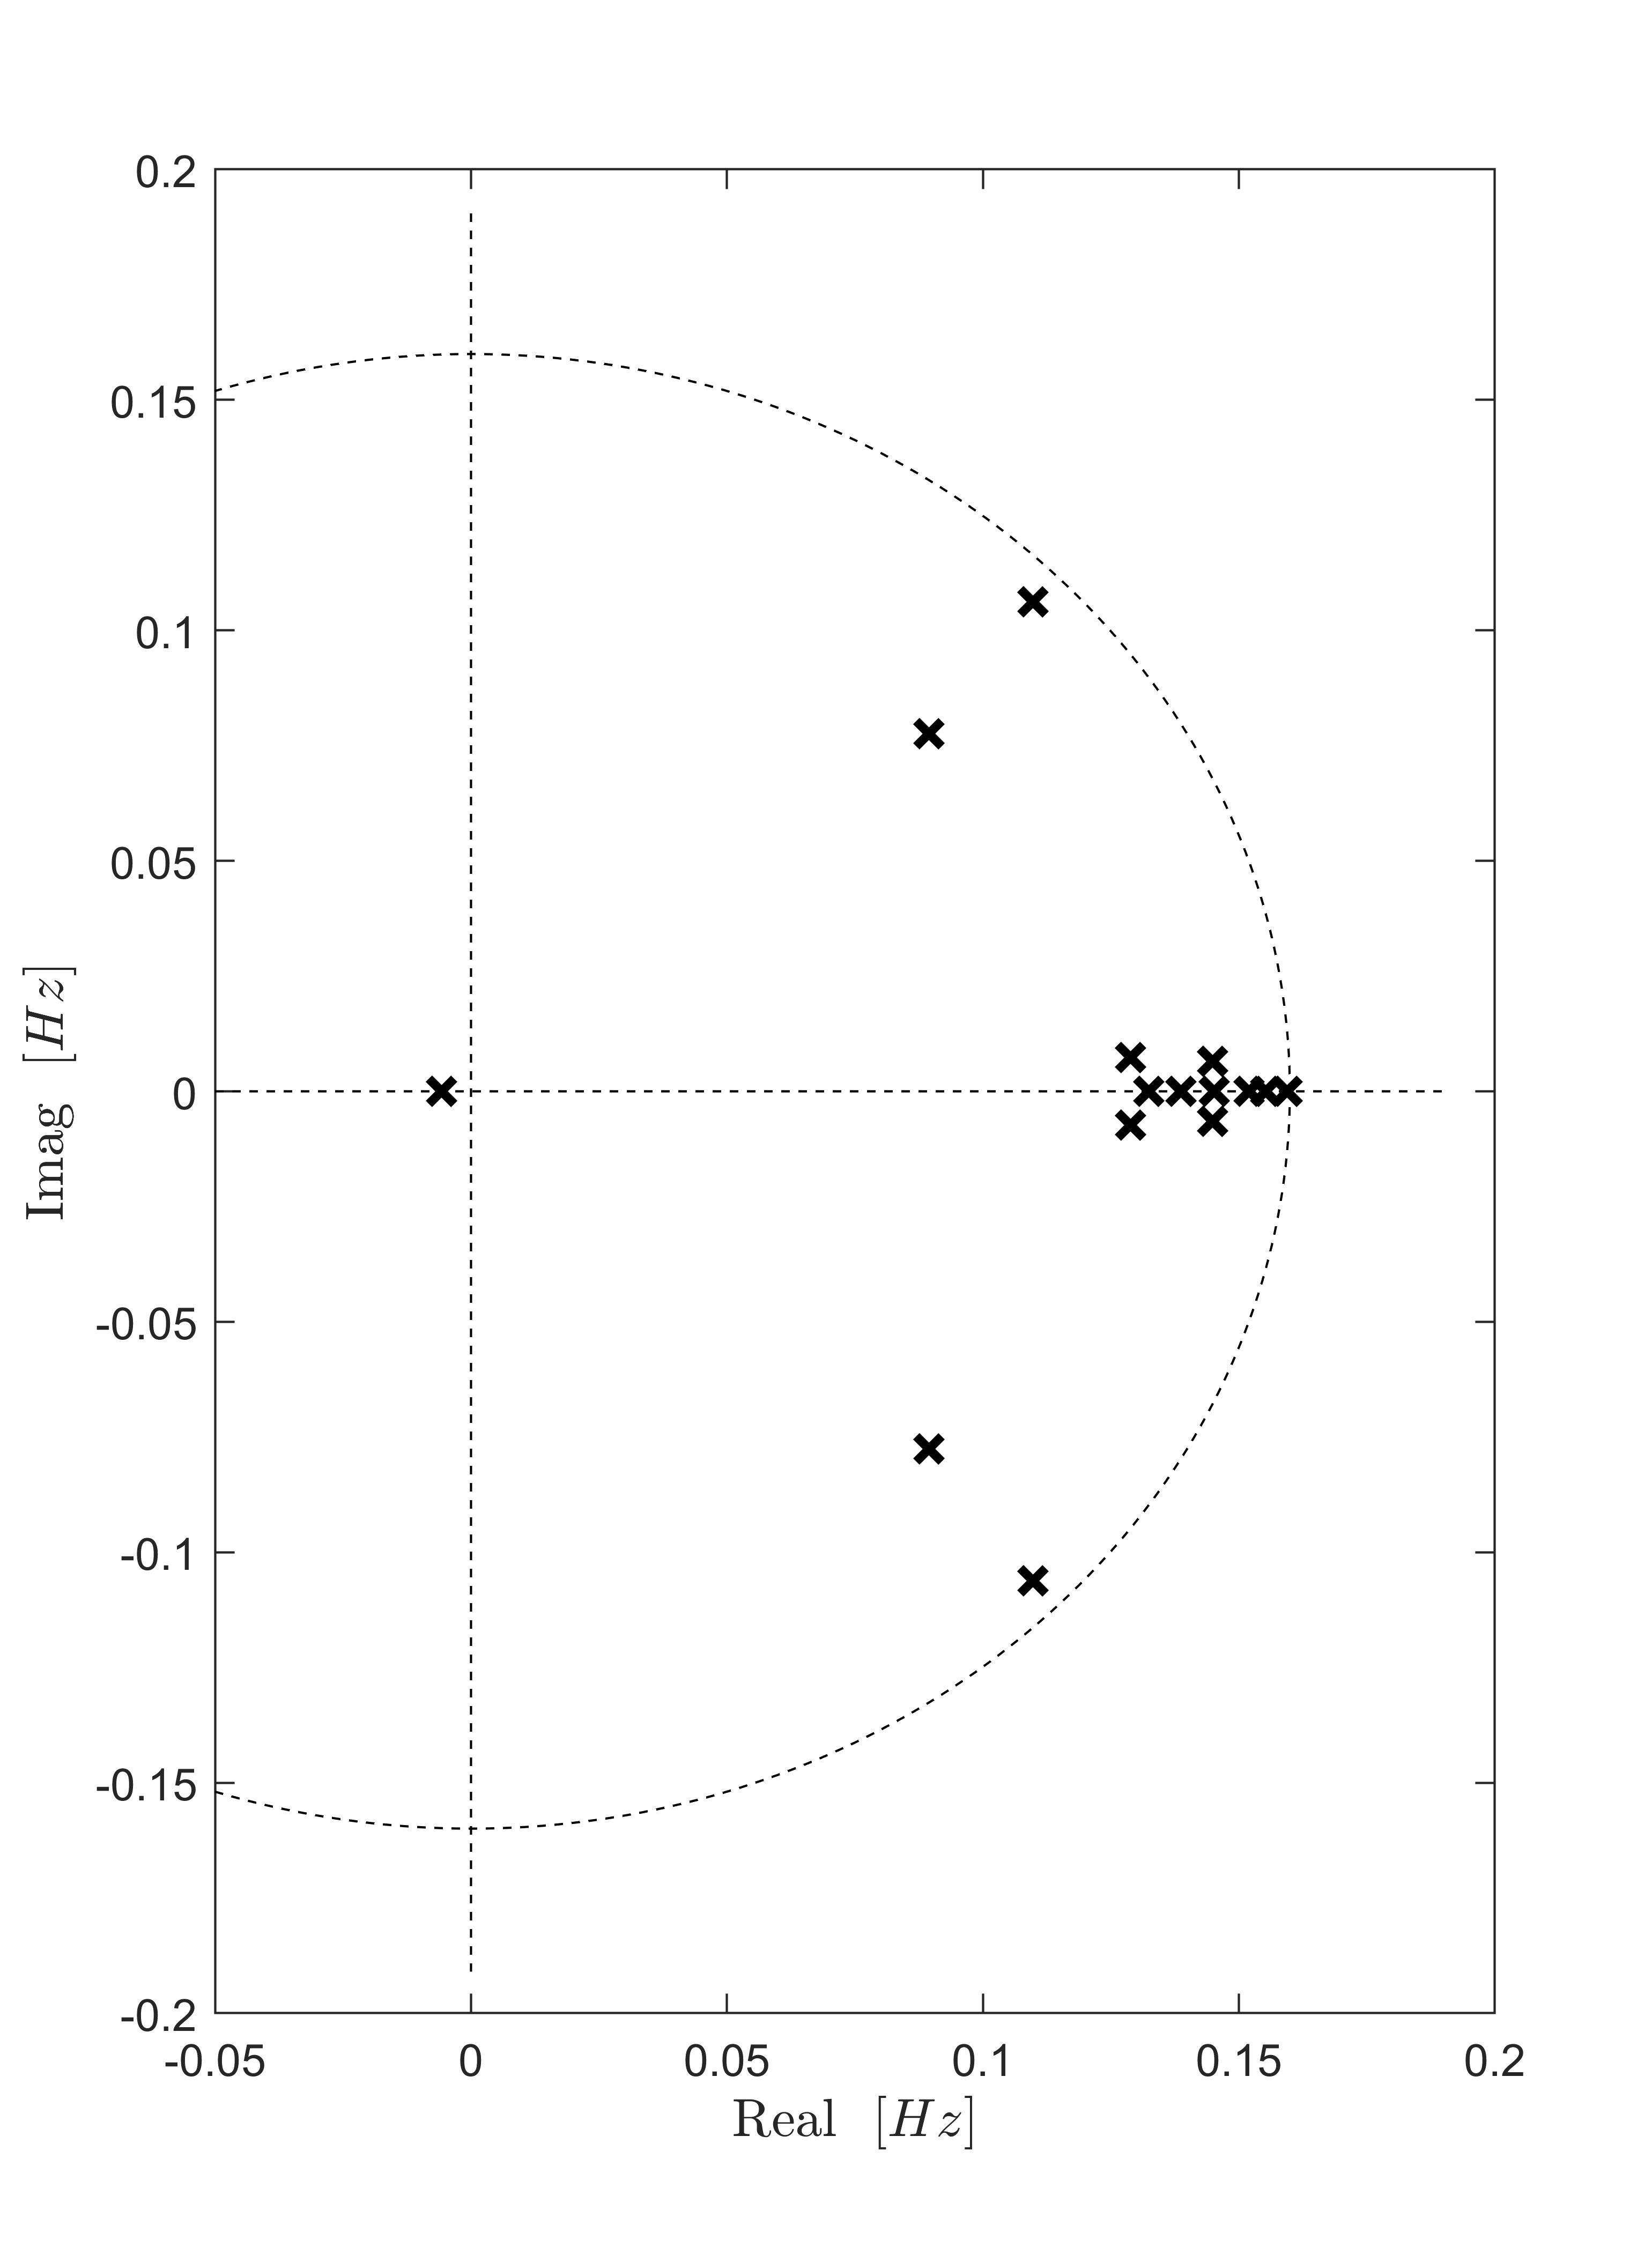
\includegraphics[width=\textwidth]{trabalho-graduacao/capitulos/figures/cap_4/Closed-Loop-Poles/ClosedLoopPoles-VLVF.png}
    \label{fig:CloseLoopPoles}
\end{figure}

	
	% 5 - Conclusões
	% ----------------------------------------------------------
\chapter{Conclusões e Trabalhos Futuros}\label{cap:conclusões}
% ----------------------------------------------------------

Foi apresentado uma metodologia para projeto de um controlador em malha fechada para sistemas aeroservoelásticos com objetivo de supressão do fenômeno de \textit{flutter}. Para isso, foi necessário modelar o sistema físico, que consiste de uma seção transversal bidimensional de asa com \textit{flap} no bordo de fuga, o que foi realizado no considerando os esforços de inércia, aerodinâmicos elásticos e externos. Em particular, os esforços aerodinâmicos dependentes da frequência reduzida foram aproximados utilizando-se de uma técnica conhecida como \glsxtrfull{RFA}, considerando quatro polos de atraso para modelar os efeitos não-estacionários. O modelo resultante foi representado no espaço de estados, o que facilitou o projeto do vetor de realimentação de estados. No presente trabalho, adotou-se o \gls{LQR} no projeto da realimentação, devido às interessantes margens de estabilidade proporcionadas.

Os resultados apresentados no capítulo anterior destacam a convergência dos resultados obtidos de característica aeroelástica do modelo com os disponíveis em literatura para o mesmo sistema. A velocidade de \textit{flutter} estimada apresentou erro percentual de apenas $2\%$ em relação ao mostrado por \textcite{book:Fung}, indicando adequação da metodologia para modelagem no domínio do tempo realizada. Esse erro pode ser justificado devido à técnica distinta para modelagem da aerodinâmica não-estacionária.

Os resultados evidenciaram a capacidade da estrutura em malha fechada proposta em estabilizar o sistema na condição de projeto, determinada como sendo o ponto de instabilidade dinâmica do sistema, ou seja, a velocidade de \textit{flutter} em malha aberta. Além disso, percebeu-se como consequência, o aumento da velocidade de \textit{flutter} do sistema em malha fechada, apesar desse aumento não ser garantido teoricamente pela formulação da lei de controle. Observou-se também o efeito desestabilizante da estrutura em malha fechada para velocidades significativamente menores do que a de projeto, introduzindo um modo de divergência no sistema. Esse efeito pode ser derivado da frequência de atuação da superfície de controle, levando o sistema a divergir de seu ponto de equilíbrio quando os esforços aerodinâmicos apresentam influência reduzida, podendo ser objeto de investigação de futuros trabalhos.

Ademais, propõe-se avaliar futuramente resultados da metodologia descrita para sistemas mais complexos, como o de uma asa 3-D, determinando-se as características modais e aerodinâmicas para as frequências de interesse e identificando os efeitos da estrutura de controle nesse sistema. Além disso, técnicas de controle mais modernas podem ser empregadas visando tratar restrições sobre o canal de entrada, que é comum em implementações práticas em sistemas de controle.

% ----------------------------------------------------------


	% Elementos pós-textuais
	\postextual
	
	
	% Referências bibliográficas
	\begingroup
	    \printbibliography[title=REFERÊNCIAS]
	\endgroup
	
	
	
	%Reconfiguração do título para apêndices e anexos
	 \renewcommand{\ABNTEXchapterupperifneeded}[1]{#1} 
	\makeatletter
	\settocpreprocessor{chapter}{%
      \let\tempf@rtoc\f@rtoc%
      \def\f@rtoc{%
      \texorpdfstring{{\tempf@rtoc}}{\tempf@rtoc}}%
      }
    \makeatother
	
	
	% Apêndices
    \begin{apendicesenv}
    	%\partapendices*
    	\selectlanguage{brazil}
    	% ----------------------------------------------------------
\chapter{Metodologia para determinação dos esforços aerodinâmicos e matrizes \textbf{AIC}s}   %Apenas a primeira letra deve ser maiúscula
% ----------------------------------------------------------

As matrizes aerodinâmicas \gls{AICa} e \gls{AICc} foram determinadas utilizando-se da metodologia apresentada por \textcite{book:Bisplinghoff} utilizando as funções de \textit{Theodorsen} para uma seção típica bidimensional. A função de Theodorsen $C(k)$ adiciona os efeitos não-estacionários aos esforços aerodinâmicos atuando sobre a seção típica devido à dependência da frequência reduzida. O comportamento da função $C(k)$ é dado conforme mostrado na Figura \ref{fig:Theodorsen}.

\begin{figure}[ht!]
    \centering
    \caption{Função de Theodorsen $C(k)$ dependente da frequência reduzida}
    \noindent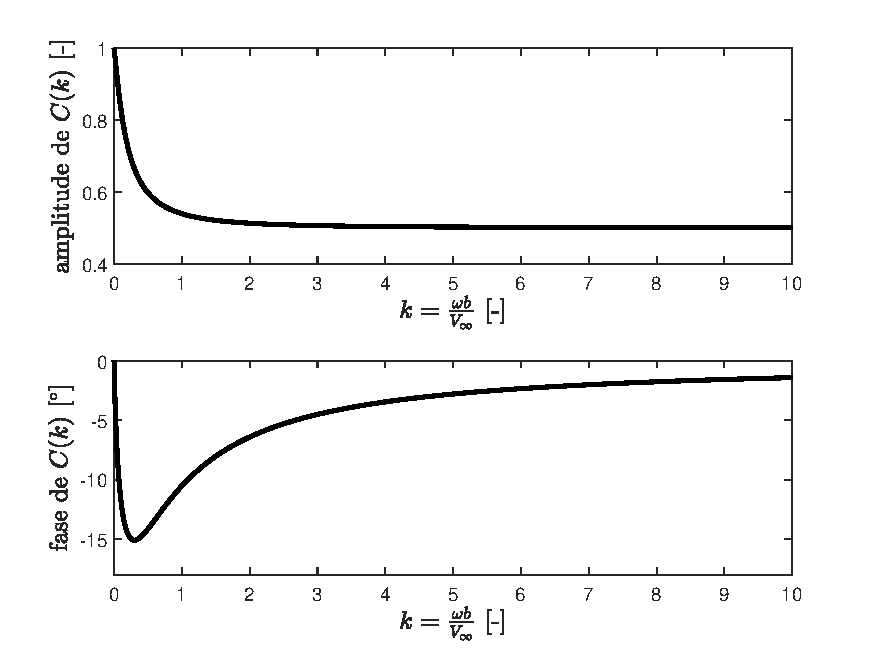
\includegraphics[width=\textwidth]{trabalho-graduacao/capitulos/figures/apendice/theodorsen.pdf}
    \label{fig:Theodorsen}
\end{figure}

Os esforços atuantes no sistema descrito na seção \ref{sec:descricao-sistema} são a sustentação $l$ e momento em torno do eixo elástico $m_{ea}$. Ambos esforços são dependentes dos parâmetros geométricos do sistema, das condições de voo para a qual são calculadas e da função de \textit{Theodorsen}. Matematicamente, são representados como

\begin{equation}\label{eq:sustentacao}
    l = 2\pi\gls{rho}\gls{Voo}\gls{b}QC(k) + \pi\gls{rho}\gls{b}^{2}\left[ \ddot{\gls{h}} + \gls{Voo}\dot{\gls{theta}} - \gls{b}\gls{a}\ddot{\gls{theta}} \right] + l_{\delta}
\end{equation}

\begin{multline}\label{eq:momento-ea}
    m_{ea} = -2\pi\gls{rho}\gls{Voo}\gls{b}^{2}Q\left\{ \frac{1}{2} - \left( a + \frac{1}{2} \right)C(k) \right\} \\ + \pi\gls{rho}\gls{b}^{2}\left[ \gls{Voo}\dot{\gls{h}} + \gls{b}\gls{a}\ddot{\gls{h}} + \gls{Voo}^{2}\gls{theta} - \gls{b}^{2}\left( \frac{1}{8}+\gls{a}^{2} \right) \ddot{\gls{theta}} \right] + m_{\delta}^{ea}
\end{multline}

\noindent em que $Q$ é uma função dependente do movimento oscilatório dos \gls{GDL}s do sistema e é dada por

\begin{multline}\label{eq:funcaoQ}
    Q = \gls{Voo}\gls{theta} + \dot{\gls{h}} + \gls{b}\left( \frac{1}{2} - \gls{a} \right)\dot{\gls{theta}} + \gls{delta}\frac{\gls{Voo}}{\pi}\left[ \sqrt{1-\gls{e}^{2}} + \cos^{-1}{\gls{e}} \right] \\ + \dot{\gls{delta}}\frac{\gls{b}}{2\pi}\left[ \left( 1 - 2\gls{e} \right)\cos^{-1}{\gls{e}} + (2-\gls{e})\sqrt{1-\gls{e}^{2}}\right]  
\end{multline}

Nas definições dos esforços aerodinâmicos em \eqref{eq:sustentacao} e \eqref{eq:momento-ea}, nota-se os termos da sustentação e momento em torno do eixo elástico decorrente da deflexão da superfície de controle, respectivamente $l_{\delta}$ e $m_{\delta}^{ea}$. Essas parcelas são calculadas como


\begin{align}\label{eq:sustentacao-delta}
\begin{split}
    l_{\delta} = &-\gls{rho}\gls{b}^{2}\gls{Voo} \left[ \gls{e}\sqrt{1-\gls{e}^{2}}-\cos^{-1}{\gls{e}} - \cos^{-1}{\gls{e}} \right]\dot{\gls{delta}} \\ &- \gls{rho}\gls{b}^{3}\left[ \gls{e}\cos^{-1}{\gls{e}} - \frac{1}{3}\left(2 + \gls{e}^{2} \right)\sqrt{1-\gls{e}^{2}} \right]\ddot{\gls{delta}}
\end{split}
\end{align}

\begin{align}\label{eq:momento-delta}
\begin{split}
    m_{\delta}^{ea} = &-\gls{rho}\gls{b}^{2}\gls{Voo}^{2} \left[ \gls{e}\sqrt{1-\gls{e}^{2}}-\cos^{-1}{\gls{e}} \right]\gls{delta} \\
        &-\gls{rho}\gls{b}^{3}\gls{Voo} \left\{ \frac{1}{3}\sqrt{1-\gls{e}^{2}}\left(\gls{e}^{2}-1\right) - \left(\gls{e}-\gls{a}\right)\left[ \gls{e}\sqrt{1-\gls{e}^{2}}-\cos^{-1}{\gls{e}} \right] \right\}\dot{\gls{delta}} \\
        &-\gls{rho}\gls{b}^{4}\left\{ \left(\frac{1}{8}+\gls{e}^{2}\right)\cos^{-1}{\gls{e}} -  \frac{1}{8}\gls{e}\sqrt{1-\gls{e}^{2}}\left(7+2\gls{e}^{2}\right) \right. \\ &+  \left. \left(\gls{e}-\gls{a}\right)\left[\frac{1}{3}\sqrt{1-\gls{e}^{2}}\left(2+\gls{e}^{2}\right) - \gls{c}\cos^{-1}{\gls{e}} \right] \right\} \ddot{\gls{delta}}
\end{split}
\end{align}

Substituindo \eqref{eq:funcaoQ}, \eqref{eq:sustentacao-delta} e \eqref{eq:momento-delta} em \eqref{eq:sustentacao} e \eqref{eq:momento-ea} é possível reescrever as expressões que indicam os esforços aerodinâmicos atuantes no sistema de forma matricial, como

\begin{equation}\label{eq:esforcos-matricial}
    \begin{bmatrix}
        l \\ m_{ea}
    \end{bmatrix} = 
    \boldsymbol{X}_{GDL,2}
    \begin{bmatrix}
        \ddot{\gls{h}} \\ \ddot{\gls{theta}}
    \end{bmatrix} +
    \boldsymbol{X}_{GDL,1}
    \begin{bmatrix}
        \dot{\gls{h}} \\ \dot{\gls{theta}}
    \end{bmatrix} +
    \boldsymbol{X}_{GDL,0}
    \begin{bmatrix}
        \gls{h} \\ \gls{theta}
    \end{bmatrix} +
    \boldsymbol{X}_{\delta,2}\ddot{\gls{delta}} + \boldsymbol{X}_{\delta,1}\dot{\gls{delta}} + \boldsymbol{X}_{\delta,0}\gls{delta}
\end{equation}

\noindent em que, $\boldsymbol{X}_{GDL,i}$ e $\boldsymbol{X}_{\delta,i}, \ i = 0,\ 1,\ 2$, representam as matrizes cujos termos são as parcelas que multiplicam cada variável dos \gls{GDL}s ou da deflexão da superfície de controle em \eqref{eq:sustentacao}, \eqref{eq:momento-ea}, \eqref{eq:funcaoQ}, \eqref{eq:sustentacao-delta} e \eqref{eq:momento-delta}. Aplicando a transformada de Laplace, \eqref{eq:esforcos-matricial} pode ser escrita como

\begin{equation}\label{eq:esforcos-matricial2}
    \begin{bmatrix}
        l \\ m_{ea}
    \end{bmatrix} = \left(
    \boldsymbol{X}_{GDL,2}s^{2} + \boldsymbol{X}_{GDL,1}s + \boldsymbol{X}_{GDL,0} \right)
    \begin{bmatrix}
        \gls{h}(s) \\ \gls{theta}(s)
    \end{bmatrix} +
    \left( \boldsymbol{X}_{\delta,2}s^{2} + \boldsymbol{X}_{\delta,1}s + \boldsymbol{X}_{\delta,0} \right) \gls{delta}(s)
\end{equation}

Utilizando da definição da frequência reduzida em \eqref{eq:Frequencia-reduzida}, pode reescrever \eqref{eq:esforcos-matricial2} como

\begin{align}\label{eq:esforcos-matricial3}
\begin{split}
    \begin{bmatrix}
        l \\ m_{ea}
    \end{bmatrix} = &\left(
    \left(\frac{\gls{Voo}}{b}\right)^{2}\boldsymbol{X}_{GDL,2}(ik)^{2} + \frac{\gls{Voo}}{b}\boldsymbol{X}_{GDL,1}(ik) + \boldsymbol{X}_{GDL,0} \right)
    \begin{bmatrix}
        \gls{h}(s) \\ \gls{theta}(s)
    \end{bmatrix} \\ &+
    \left( \left(\frac{\gls{Voo}}{b}\right)^{2}\boldsymbol{X}_{\delta,2}(ik)^{2} + \frac{\gls{Voo}}{b}\boldsymbol{X}_{\delta,1}(ik) + \boldsymbol{X}_{\delta,0} \right) \gls{delta}(s)
\end{split}
\end{align}

Analisando \eqref{eq:esforcos-matricial3} em comparação com o lado direito de \eqref{eq:equacao-dinamica-final}, percebe-se que, organizando os termos e colocando a pressão dinâmica $\gls{qoo}$ em evidência em \eqref{eq:esforcos-matricial3}, encontramos as matrizes $\gls{AICa}$ e $\gls{AICc}$ como

\begin{equation}\label{eq:AICa-definica}
    \gls{AICa} = \frac{1}{\gls{qoo}}\left(
    \left(\frac{\gls{Voo}}{b}\right)^{2}\boldsymbol{X}_{GDL,2}(ik)^{2} + \frac{\gls{Voo}}{b}\boldsymbol{X}_{GDL,1}(ik) + \boldsymbol{X}_{GDL,0} \right)
\end{equation}

\begin{equation}\label{eq:AICc-definica}
    \gls{AICc} = \frac{1}{\gls{qoo}}\left( \left(\frac{\gls{Voo}}{b}\right)^{2}\boldsymbol{X}_{\delta,2}(ik)^{2} + \frac{\gls{Voo}}{b}\boldsymbol{X}_{\delta,1}(ik) + \boldsymbol{X}_{\delta,0} \right)
\end{equation}

    \end{apendicesenv}

    % Anexos
    %\begin{anexosenv}
        %\partanexos*
    	%% ----------------------------------------------------------
\chapter{Descrição}   %Apenas a primeira letra deve ser maiúscula
% ----------------------------------------------------------

São documentos não elaborados pelo autor que servem como fundamentação (mapas, leis, estatutos). Deve ser precedido da palavra ANEXO, identificada por letras maiúsculas consecutivas, travessão e pelo respectivo título. Utilizam-se letras maiúsculas dobradas quando esgotadas as letras do alfabeto. 

    %\end{anexosenv}

\end{document}